\PassOptionsToPackage{unicode=true}{hyperref} % options for packages loaded elsewhere
\PassOptionsToPackage{hyphens}{url}
%
\documentclass[]{book}
\usepackage{lmodern}
\usepackage{amssymb,amsmath}
\usepackage{ifxetex,ifluatex}
\usepackage{fixltx2e} % provides \textsubscript
\ifnum 0\ifxetex 1\fi\ifluatex 1\fi=0 % if pdftex
  \usepackage[T1]{fontenc}
  \usepackage[utf8]{inputenc}
  \usepackage{textcomp} % provides euro and other symbols
\else % if luatex or xelatex
  \usepackage{unicode-math}
  \defaultfontfeatures{Ligatures=TeX,Scale=MatchLowercase}
\fi
% use upquote if available, for straight quotes in verbatim environments
\IfFileExists{upquote.sty}{\usepackage{upquote}}{}
% use microtype if available
\IfFileExists{microtype.sty}{%
\usepackage[]{microtype}
\UseMicrotypeSet[protrusion]{basicmath} % disable protrusion for tt fonts
}{}
\IfFileExists{parskip.sty}{%
\usepackage{parskip}
}{% else
\setlength{\parindent}{0pt}
\setlength{\parskip}{6pt plus 2pt minus 1pt}
}
\usepackage{hyperref}
\hypersetup{
            pdftitle={Supplemental Material},
            pdfauthor={Alexander Lalejini, Austin J. Ferguson, and Charles Ofria},
            pdfborder={0 0 0},
            breaklinks=true}
\urlstyle{same}  % don't use monospace font for urls
\usepackage{color}
\usepackage{fancyvrb}
\newcommand{\VerbBar}{|}
\newcommand{\VERB}{\Verb[commandchars=\\\{\}]}
\DefineVerbatimEnvironment{Highlighting}{Verbatim}{commandchars=\\\{\}}
% Add ',fontsize=\small' for more characters per line
\usepackage{framed}
\definecolor{shadecolor}{RGB}{248,248,248}
\newenvironment{Shaded}{\begin{snugshade}}{\end{snugshade}}
\newcommand{\AlertTok}[1]{\textcolor[rgb]{0.94,0.16,0.16}{#1}}
\newcommand{\AnnotationTok}[1]{\textcolor[rgb]{0.56,0.35,0.01}{\textbf{\textit{#1}}}}
\newcommand{\AttributeTok}[1]{\textcolor[rgb]{0.77,0.63,0.00}{#1}}
\newcommand{\BaseNTok}[1]{\textcolor[rgb]{0.00,0.00,0.81}{#1}}
\newcommand{\BuiltInTok}[1]{#1}
\newcommand{\CharTok}[1]{\textcolor[rgb]{0.31,0.60,0.02}{#1}}
\newcommand{\CommentTok}[1]{\textcolor[rgb]{0.56,0.35,0.01}{\textit{#1}}}
\newcommand{\CommentVarTok}[1]{\textcolor[rgb]{0.56,0.35,0.01}{\textbf{\textit{#1}}}}
\newcommand{\ConstantTok}[1]{\textcolor[rgb]{0.00,0.00,0.00}{#1}}
\newcommand{\ControlFlowTok}[1]{\textcolor[rgb]{0.13,0.29,0.53}{\textbf{#1}}}
\newcommand{\DataTypeTok}[1]{\textcolor[rgb]{0.13,0.29,0.53}{#1}}
\newcommand{\DecValTok}[1]{\textcolor[rgb]{0.00,0.00,0.81}{#1}}
\newcommand{\DocumentationTok}[1]{\textcolor[rgb]{0.56,0.35,0.01}{\textbf{\textit{#1}}}}
\newcommand{\ErrorTok}[1]{\textcolor[rgb]{0.64,0.00,0.00}{\textbf{#1}}}
\newcommand{\ExtensionTok}[1]{#1}
\newcommand{\FloatTok}[1]{\textcolor[rgb]{0.00,0.00,0.81}{#1}}
\newcommand{\FunctionTok}[1]{\textcolor[rgb]{0.00,0.00,0.00}{#1}}
\newcommand{\ImportTok}[1]{#1}
\newcommand{\InformationTok}[1]{\textcolor[rgb]{0.56,0.35,0.01}{\textbf{\textit{#1}}}}
\newcommand{\KeywordTok}[1]{\textcolor[rgb]{0.13,0.29,0.53}{\textbf{#1}}}
\newcommand{\NormalTok}[1]{#1}
\newcommand{\OperatorTok}[1]{\textcolor[rgb]{0.81,0.36,0.00}{\textbf{#1}}}
\newcommand{\OtherTok}[1]{\textcolor[rgb]{0.56,0.35,0.01}{#1}}
\newcommand{\PreprocessorTok}[1]{\textcolor[rgb]{0.56,0.35,0.01}{\textit{#1}}}
\newcommand{\RegionMarkerTok}[1]{#1}
\newcommand{\SpecialCharTok}[1]{\textcolor[rgb]{0.00,0.00,0.00}{#1}}
\newcommand{\SpecialStringTok}[1]{\textcolor[rgb]{0.31,0.60,0.02}{#1}}
\newcommand{\StringTok}[1]{\textcolor[rgb]{0.31,0.60,0.02}{#1}}
\newcommand{\VariableTok}[1]{\textcolor[rgb]{0.00,0.00,0.00}{#1}}
\newcommand{\VerbatimStringTok}[1]{\textcolor[rgb]{0.31,0.60,0.02}{#1}}
\newcommand{\WarningTok}[1]{\textcolor[rgb]{0.56,0.35,0.01}{\textbf{\textit{#1}}}}
\usepackage{longtable,booktabs}
% Fix footnotes in tables (requires footnote package)
\IfFileExists{footnote.sty}{\usepackage{footnote}\makesavenoteenv{longtable}}{}
\usepackage{graphicx,grffile}
\makeatletter
\def\maxwidth{\ifdim\Gin@nat@width>\linewidth\linewidth\else\Gin@nat@width\fi}
\def\maxheight{\ifdim\Gin@nat@height>\textheight\textheight\else\Gin@nat@height\fi}
\makeatother
% Scale images if necessary, so that they will not overflow the page
% margins by default, and it is still possible to overwrite the defaults
% using explicit options in \includegraphics[width, height, ...]{}
\setkeys{Gin}{width=\maxwidth,height=\maxheight,keepaspectratio}
\setlength{\emergencystretch}{3em}  % prevent overfull lines
\providecommand{\tightlist}{%
  \setlength{\itemsep}{0pt}\setlength{\parskip}{0pt}}
\setcounter{secnumdepth}{5}
% Redefines (sub)paragraphs to behave more like sections
\ifx\paragraph\undefined\else
\let\oldparagraph\paragraph
\renewcommand{\paragraph}[1]{\oldparagraph{#1}\mbox{}}
\fi
\ifx\subparagraph\undefined\else
\let\oldsubparagraph\subparagraph
\renewcommand{\subparagraph}[1]{\oldsubparagraph{#1}\mbox{}}
\fi

% set default figure placement to htbp
\makeatletter
\def\fps@figure{htbp}
\makeatother

\usepackage[]{natbib}
\bibliographystyle{apalike}

\title{Supplemental Material}
\author{Alexander Lalejini, Austin J. Ferguson, and Charles Ofria}
\date{2021-01-19}

\begin{document}
\maketitle

{
\setcounter{tocdepth}{1}
\tableofcontents
}
\hypertarget{introduction}{%
\chapter{Introduction}\label{introduction}}

TODO

\hypertarget{validation-experiment}{%
\chapter{Validation experiment}\label{validation-experiment}}

In this experiment, we validate that
(1) we observe the evolution of phenotypic plasticity in a changing environment when digital organisms have access to sensory instructions (capable of differentiating environmental states)
and (2) that adaptive phenotypic plasticity does not evolve when populations lack access to sensory instructions.

\hypertarget{overview}{%
\section{Overview}\label{overview}}

\begin{Shaded}
\begin{Highlighting}[]
\NormalTok{total_updates <-}\StringTok{ }\DecValTok{200000}
\NormalTok{replicates <-}\StringTok{ }\DecValTok{100}

\NormalTok{all_traits <-}\StringTok{ }\KeywordTok{c}\NormalTok{(}\StringTok{"not"}\NormalTok{,}\StringTok{"nand"}\NormalTok{,}\StringTok{"and"}\NormalTok{,}\StringTok{"ornot"}\NormalTok{,}\StringTok{"or"}\NormalTok{,}\StringTok{"andnot"}\NormalTok{)}
\NormalTok{traits_set_a <-}\StringTok{ }\KeywordTok{c}\NormalTok{(}\StringTok{"not"}\NormalTok{, }\StringTok{"and"}\NormalTok{, }\StringTok{"or"}\NormalTok{)}
\NormalTok{traits_set_b <-}\StringTok{ }\KeywordTok{c}\NormalTok{(}\StringTok{"nand"}\NormalTok{, }\StringTok{"ornot"}\NormalTok{, }\StringTok{"andnot"}\NormalTok{)}

\CommentTok{# Relative location of data.}
\NormalTok{working_directory <-}\StringTok{ "experiments/2021-01-07-validation/analysis/"} \CommentTok{# << For bookdown}
\CommentTok{# working_directory <- "./"                                              # << For local analysis}
\end{Highlighting}
\end{Shaded}

We evolved populations of digital organisms under four conditions:

\begin{enumerate}
\def\labelenumi{\arabic{enumi}.}
\tightlist
\item
  A fluctuating environment with access to sensory instructions
\item
  A fluctuating environment without access to sensory instructions (i.e., sensory instructions are no-operations)
\item
  A constant environment with access to sensory instructions
\item
  A constant environment without access to sensory instructions
\end{enumerate}

In fluctuating environments, we alternate between rewarding and punishing different sets of computational tasks.
In one environment, we reward tasks not, and, or and punish tasks nand, ornot, andnot.
In the alternative environment, we reward tasks nand, ornot, andnot and punish tasks not, and, or.
In constant environments, we reward all tasks (not, nand, and, ornot, or, andnot).

For each replicate of each condition, we extract the dominant (i.e., most numerous) genotype at the end of the run to analyze further.
We expect to observe the evolution of adaptive phenotypic plasticity in only the first experimental condition.
In conditions without sensors, plasticity in any form should be unable to evolve.

\hypertarget{analysis-dependencies}{%
\section{Analysis dependencies}\label{analysis-dependencies}}

Load all required R libraries.

\begin{Shaded}
\begin{Highlighting}[]
\KeywordTok{library}\NormalTok{(ggplot2)}
\KeywordTok{library}\NormalTok{(tidyverse)}
\KeywordTok{library}\NormalTok{(cowplot)}
\KeywordTok{source}\NormalTok{(}\StringTok{"https://gist.githubusercontent.com/benmarwick/2a1bb0133ff568cbe28d/raw/fb53bd97121f7f9ce947837ef1a4c65a73bffb3f/geom_flat_violin.R"}\NormalTok{)}
\end{Highlighting}
\end{Shaded}

These analyses were conducted/knitted with the following computing environment:

\begin{Shaded}
\begin{Highlighting}[]
\KeywordTok{print}\NormalTok{(version)}
\end{Highlighting}
\end{Shaded}

\begin{verbatim}
##                _                           
## platform       x86_64-pc-linux-gnu         
## arch           x86_64                      
## os             linux-gnu                   
## system         x86_64, linux-gnu           
## status                                     
## major          4                           
## minor          0.3                         
## year           2020                        
## month          10                          
## day            10                          
## svn rev        79318                       
## language       R                           
## version.string R version 4.0.3 (2020-10-10)
## nickname       Bunny-Wunnies Freak Out
\end{verbatim}

\hypertarget{setup}{%
\section{Setup}\label{setup}}

\begin{Shaded}
\begin{Highlighting}[]
\NormalTok{data_loc <-}\StringTok{ }\KeywordTok{paste0}\NormalTok{(working_directory, }\StringTok{"data/aggregate.csv"}\NormalTok{)}
\NormalTok{data <-}\StringTok{ }\KeywordTok{read.csv}\NormalTok{(data_loc, }\DataTypeTok{na.strings=}\StringTok{"NONE"}\NormalTok{)}

\NormalTok{data}\OperatorTok{$}\NormalTok{DISABLE_REACTION_SENSORS <-}\StringTok{ }\KeywordTok{as.factor}\NormalTok{(data}\OperatorTok{$}\NormalTok{DISABLE_REACTION_SENSORS)}
\NormalTok{data}\OperatorTok{$}\NormalTok{chg_env <-}\StringTok{ }\KeywordTok{as.factor}\NormalTok{(data}\OperatorTok{$}\NormalTok{chg_env)}
\NormalTok{data}\OperatorTok{$}\NormalTok{dom_plastic_odd_even <-}\StringTok{ }\KeywordTok{as.factor}\NormalTok{(data}\OperatorTok{$}\NormalTok{dom_plastic_odd_even)}
\NormalTok{data}\OperatorTok{$}\NormalTok{sensors <-}\StringTok{ }\NormalTok{data}\OperatorTok{$}\NormalTok{DISABLE_REACTION_SENSORS }\OperatorTok{==}\StringTok{ "0"}
\NormalTok{data}\OperatorTok{$}\NormalTok{is_plastic <-}\StringTok{ }\NormalTok{data}\OperatorTok{$}\NormalTok{dom_plastic_odd_even }\OperatorTok{==}\StringTok{ "True"}

\NormalTok{env_label_fun <-}\StringTok{ }\ControlFlowTok{function}\NormalTok{(chg_env) \{}
  \ControlFlowTok{if}\NormalTok{ (chg_env) \{}
    \KeywordTok{return}\NormalTok{(}\StringTok{"Fluctuating"}\NormalTok{)}
\NormalTok{  \} }\ControlFlowTok{else}\NormalTok{ \{}
    \KeywordTok{return}\NormalTok{(}\StringTok{"Constant"}\NormalTok{)}
\NormalTok{  \}}
\NormalTok{\}}

\NormalTok{sensors_label_fun <-}\StringTok{ }\ControlFlowTok{function}\NormalTok{(has_sensors) \{}
  \ControlFlowTok{if}\NormalTok{ (has_sensors) \{}
    \KeywordTok{return}\NormalTok{(}\StringTok{"Sensors"}\NormalTok{)}
\NormalTok{  \} }\ControlFlowTok{else}\NormalTok{ \{}
    \KeywordTok{return}\NormalTok{(}\StringTok{"No sensors"}\NormalTok{)}
\NormalTok{  \}}
\NormalTok{\}}

\CommentTok{# Count observed plasticity for each condition (I'm sure there's a 'tidier' way to do this..)}
\NormalTok{observed_plasticity <-}\StringTok{ }\KeywordTok{data.frame}\NormalTok{(}
  \DataTypeTok{environment=}\KeywordTok{character}\NormalTok{(),}
  \DataTypeTok{sensors=}\KeywordTok{character}\NormalTok{(),}
  \DataTypeTok{plastic=}\KeywordTok{integer}\NormalTok{(),}
  \DataTypeTok{nonplastic=}\KeywordTok{integer}\NormalTok{(),}
  \DataTypeTok{plastic_adaptive=}\KeywordTok{integer}\NormalTok{(),}
  \DataTypeTok{plastic_optimal=}\KeywordTok{integer}\NormalTok{(),}
  \DataTypeTok{plastic_nonadaptive=}\KeywordTok{integer}\NormalTok{()}
\NormalTok{)}
\ControlFlowTok{for}\NormalTok{ (env_chg }\ControlFlowTok{in} \KeywordTok{levels}\NormalTok{(data}\OperatorTok{$}\NormalTok{chg_env)) \{}
  \ControlFlowTok{for}\NormalTok{ (disabled_sensors }\ControlFlowTok{in} \KeywordTok{levels}\NormalTok{(data}\OperatorTok{$}\NormalTok{DISABLE_REACTION_SENSORS)) \{}
\NormalTok{    cond_data <-}\StringTok{ }\KeywordTok{filter}\NormalTok{(data, chg_env }\OperatorTok{==}\StringTok{ }\NormalTok{env_chg }\OperatorTok{&}\StringTok{ }\NormalTok{data}\OperatorTok{$}\NormalTok{DISABLE_REACTION_SENSORS }\OperatorTok{==}\StringTok{ }\NormalTok{disabled_sensors)}
\NormalTok{    environment_label <-}\StringTok{ }\KeywordTok{env_label_fun}\NormalTok{(env_chg)}
\NormalTok{    sensors_label <-}\StringTok{ }\KeywordTok{sensors_label_fun}\NormalTok{(disabled_sensors }\OperatorTok{==}\StringTok{ "0"}\NormalTok{)}

\NormalTok{    observed_plasticity <-}\StringTok{ }\NormalTok{observed_plasticity }\OperatorTok\StringTok{ }\KeywordTok{add_row}\NormalTok{(}
      \DataTypeTok{environment=}\NormalTok{environment_label,}
      \DataTypeTok{sensors=}\NormalTok{sensors_label,}
      \DataTypeTok{plastic=}\KeywordTok{nrow}\NormalTok{(}\KeywordTok{filter}\NormalTok{(cond_data, is_plastic}\OperatorTok{==}\OtherTok{TRUE}\NormalTok{)),}
      \DataTypeTok{nonplastic=}\KeywordTok{nrow}\NormalTok{(}\KeywordTok{filter}\NormalTok{(cond_data, is_plastic}\OperatorTok{==}\OtherTok{FALSE}\NormalTok{)),}
      \DataTypeTok{plastic_adaptive=}\KeywordTok{nrow}\NormalTok{(}\KeywordTok{filter}\NormalTok{(cond_data, dom_adaptive_plasticity}\OperatorTok{==}\StringTok{"True"}\NormalTok{)),}
      \DataTypeTok{plastic_optimal=}\KeywordTok{nrow}\NormalTok{(}\KeywordTok{filter}\NormalTok{(cond_data, dom_optimal_plastic}\OperatorTok{==}\StringTok{"True"}\NormalTok{)),}
      \DataTypeTok{plastic_nonadaptive=}\KeywordTok{nrow}\NormalTok{(}\KeywordTok{filter}\NormalTok{(cond_data, is_plastic}\OperatorTok{==}\OtherTok{TRUE} \OperatorTok{&}\StringTok{ }\NormalTok{dom_adaptive_plasticity}\OperatorTok{==}\StringTok{"False"}\NormalTok{))}
\NormalTok{    )}
\NormalTok{  \}}
\NormalTok{\}}

\NormalTok{observed_plasticity <-}\StringTok{ }\KeywordTok{pivot_longer}\NormalTok{(}
\NormalTok{  observed_plasticity,}
  \DataTypeTok{cols=}\KeywordTok{c}\NormalTok{(}\StringTok{"plastic"}\NormalTok{, }\StringTok{"plastic_adaptive"}\NormalTok{, }\StringTok{"plastic_optimal"}\NormalTok{, }\StringTok{"plastic_nonadaptive"}\NormalTok{, }\StringTok{"nonplastic"}\NormalTok{),}
  \DataTypeTok{names_to=}\StringTok{"phenotype"}\NormalTok{,}
  \DataTypeTok{values_to=}\StringTok{"phenotype_cnt"}
\NormalTok{)}

\CommentTok{####### misc #######}
\CommentTok{# Configure our default graphing theme}
\KeywordTok{theme_set}\NormalTok{(}\KeywordTok{theme_cowplot}\NormalTok{())}
\end{Highlighting}
\end{Shaded}

\hypertarget{evolution-of-phenotypic-plasticity}{%
\section{Evolution of phenotypic plasticity}\label{evolution-of-phenotypic-plasticity}}

For each experimental condition, do we observe the evolution of phenotypic plasticity? To test for phenotypic plasticity, we culture digital organisms in both environments from the fluctuating condition (including organisms evolved in a constant environment).
Any plasticity that we observe from digital organisms evolved under constant conditions is cryptic variation (as these organisms were never exposed to these culturing environments).

\begin{Shaded}
\begin{Highlighting}[]
\KeywordTok{ggplot}\NormalTok{(}\KeywordTok{filter}\NormalTok{(observed_plasticity, phenotype }\OperatorTok\StringTok{ }\KeywordTok{c}\NormalTok{(}\StringTok{"plastic"}\NormalTok{, }\StringTok{"nonplastic"}\NormalTok{)), }\KeywordTok{aes}\NormalTok{(}\DataTypeTok{x=}\NormalTok{phenotype, }\DataTypeTok{y=}\NormalTok{phenotype_cnt, }\DataTypeTok{fill=}\NormalTok{phenotype)) }\OperatorTok{+}
\StringTok{  }\KeywordTok{geom_bar}\NormalTok{(}
    \DataTypeTok{stat=}\StringTok{"identity"}\NormalTok{,}
    \DataTypeTok{position=}\KeywordTok{position_dodge}\NormalTok{(}\FloatTok{0.9}\NormalTok{)}
\NormalTok{  ) }\OperatorTok{+}
\StringTok{  }\KeywordTok{geom_text}\NormalTok{(}
    \DataTypeTok{stat=}\StringTok{"identity"}\NormalTok{,}
    \DataTypeTok{mapping=}\KeywordTok{aes}\NormalTok{(}\DataTypeTok{label=}\NormalTok{phenotype_cnt),}
    \DataTypeTok{vjust=}\FloatTok{0.05}
\NormalTok{  ) }\OperatorTok{+}
\StringTok{  }\KeywordTok{scale_fill_brewer}\NormalTok{(}\DataTypeTok{palette=}\StringTok{"Accent"}\NormalTok{) }\OperatorTok{+}
\StringTok{  }\KeywordTok{scale_x_discrete}\NormalTok{(}
    \DataTypeTok{name=}\StringTok{"Phenotype"}\NormalTok{,}
    \DataTypeTok{limits=}\KeywordTok{c}\NormalTok{(}\StringTok{"plastic"}\NormalTok{, }\StringTok{"nonplastic"}\NormalTok{),}
    \DataTypeTok{labels=}\KeywordTok{c}\NormalTok{(}\StringTok{"Plastic"}\NormalTok{, }\StringTok{"Non-plastic"}\NormalTok{)}
\NormalTok{  ) }\OperatorTok{+}
\StringTok{  }\KeywordTok{facet_grid}\NormalTok{(sensors}\OperatorTok{~}\NormalTok{environment) }\OperatorTok{+}
\StringTok{  }\KeywordTok{theme}\NormalTok{(}
    \DataTypeTok{legend.position=}\StringTok{"none"}
\NormalTok{  )}
\end{Highlighting}
\end{Shaded}

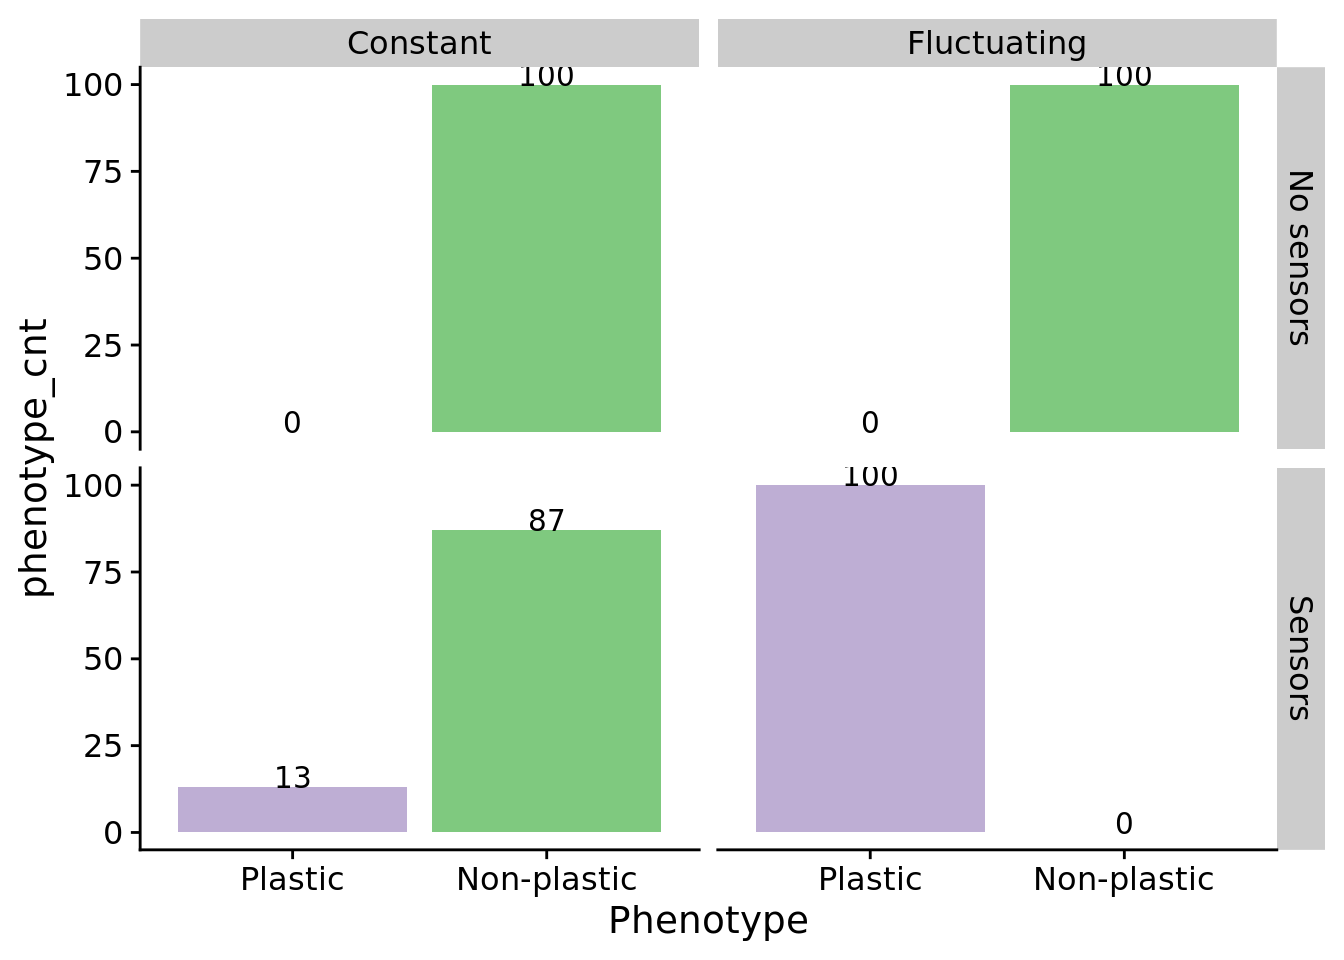
\includegraphics{supplemental-material_files/figure-latex/unnamed-chunk-5-1.pdf}

Indeed, we do not observe the evolution of phenotypic plasticity in any replicates in which digital organisms do not have access to sensory instructions.
We do observe the evolution of plasticity (not necessarily adaptive plasticity) in both constant and fluctuating environments where sensors are enabled.

To what extent is the observed phenotypic plasticity adaptive?

\begin{Shaded}
\begin{Highlighting}[]
\KeywordTok{ggplot}\NormalTok{(}\KeywordTok{filter}\NormalTok{(observed_plasticity, environment}\OperatorTok{==}\StringTok{"Fluctuating"} \OperatorTok{&}\StringTok{ }\NormalTok{sensors }\OperatorTok{==}\StringTok{ "Sensors"} \OperatorTok{&}\StringTok{ }\NormalTok{phenotype }\OperatorTok\StringTok{ }\KeywordTok{c}\NormalTok{(}\StringTok{"plastic"}\NormalTok{, }\StringTok{"plastic_adaptive"}\NormalTok{, }\StringTok{"plastic_optimal"}\NormalTok{, }\StringTok{"plastic_nonadaptive"}\NormalTok{)), }\KeywordTok{aes}\NormalTok{(}\DataTypeTok{x=}\NormalTok{phenotype, }\DataTypeTok{y=}\NormalTok{phenotype_cnt, }\DataTypeTok{fill=}\NormalTok{phenotype)) }\OperatorTok{+}
\StringTok{  }\KeywordTok{geom_bar}\NormalTok{(}
    \DataTypeTok{stat=}\StringTok{"identity"}\NormalTok{,}
    \DataTypeTok{position=}\KeywordTok{position_dodge}\NormalTok{(}\FloatTok{0.9}\NormalTok{)}
\NormalTok{  ) }\OperatorTok{+}
\StringTok{  }\KeywordTok{geom_text}\NormalTok{(}
    \DataTypeTok{stat=}\StringTok{"identity"}\NormalTok{,}
    \DataTypeTok{mapping=}\KeywordTok{aes}\NormalTok{(}\DataTypeTok{label=}\NormalTok{phenotype_cnt),}
    \DataTypeTok{vjust=}\FloatTok{0.05}
\NormalTok{  ) }\OperatorTok{+}
\StringTok{  }\KeywordTok{scale_fill_brewer}\NormalTok{(}\DataTypeTok{palette=}\StringTok{"Accent"}\NormalTok{) }\OperatorTok{+}
\StringTok{  }\KeywordTok{scale_x_discrete}\NormalTok{(}
    \DataTypeTok{name=}\StringTok{"Phenotype"}\NormalTok{,}
    \DataTypeTok{limits=}\KeywordTok{c}\NormalTok{(}\StringTok{"plastic"}\NormalTok{,  }\StringTok{"plastic_adaptive"}\NormalTok{, }\StringTok{"plastic_optimal"}\NormalTok{, }\StringTok{"plastic_nonadaptive"}\NormalTok{),}
    \DataTypeTok{labels=}\KeywordTok{c}\NormalTok{(}\StringTok{"Total plastic"}\NormalTok{, }\StringTok{"Adaptive plasticity"}\NormalTok{, }\StringTok{"Optimal plasticity"}\NormalTok{, }\StringTok{"Non-adaptive plasticity"}\NormalTok{)}
\NormalTok{  ) }\OperatorTok{+}
\StringTok{  }\KeywordTok{facet_grid}\NormalTok{(sensors}\OperatorTok{~}\NormalTok{environment) }\OperatorTok{+}
\StringTok{  }\KeywordTok{theme}\NormalTok{(}
    \DataTypeTok{legend.position=}\StringTok{"none"}
\NormalTok{  )}
\end{Highlighting}
\end{Shaded}

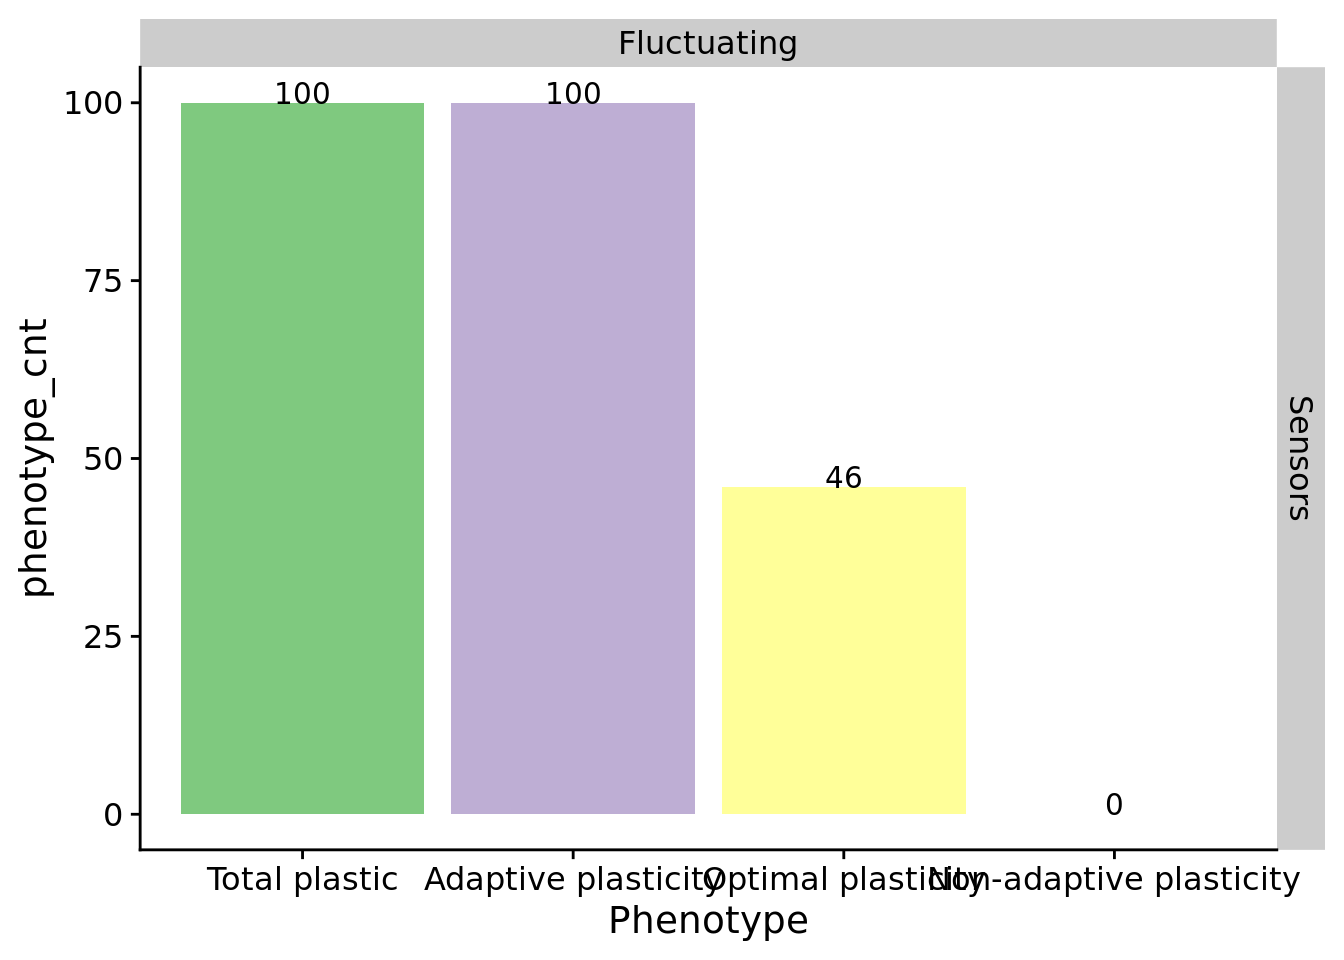
\includegraphics{supplemental-material_files/figure-latex/unnamed-chunk-6-1.pdf}

\hypertarget{effect-of-phenotypic-plasticity-on-subsequent-evolutionary-dynamics}{%
\chapter{Effect of phenotypic plasticity on subsequent evolutionary dynamics}\label{effect-of-phenotypic-plasticity-on-subsequent-evolutionary-dynamics}}

\hypertarget{overview-1}{%
\section{Overview}\label{overview-1}}

\begin{Shaded}
\begin{Highlighting}[]
\NormalTok{total_updates <-}\StringTok{ }\DecValTok{200000}
\NormalTok{replicates <-}\StringTok{ }\DecValTok{200}

\NormalTok{all_traits <-}\StringTok{ }\KeywordTok{c}\NormalTok{(}\StringTok{"not"}\NormalTok{,}\StringTok{"nand"}\NormalTok{,}\StringTok{"and"}\NormalTok{,}\StringTok{"ornot"}\NormalTok{,}\StringTok{"or"}\NormalTok{,}\StringTok{"andnot"}\NormalTok{)}
\NormalTok{traits_set_a <-}\StringTok{ }\KeywordTok{c}\NormalTok{(}\StringTok{"not"}\NormalTok{, }\StringTok{"and"}\NormalTok{, }\StringTok{"or"}\NormalTok{)}
\NormalTok{traits_set_b <-}\StringTok{ }\KeywordTok{c}\NormalTok{(}\StringTok{"nand"}\NormalTok{, }\StringTok{"ornot"}\NormalTok{, }\StringTok{"andnot"}\NormalTok{)}

\CommentTok{# Relative location of data.}
\NormalTok{working_directory <-}\StringTok{ "experiments/2021-01-12-evo-dynamics/analysis/"} \CommentTok{# << For bookdown}
\CommentTok{# working_directory <- "./"                                              # << For local analysis}
\end{Highlighting}
\end{Shaded}

\hypertarget{analysis-dependencies-1}{%
\section{Analysis dependencies}\label{analysis-dependencies-1}}

Load all required R libraries.

\begin{Shaded}
\begin{Highlighting}[]
\KeywordTok{library}\NormalTok{(ggplot2)}
\KeywordTok{library}\NormalTok{(tidyverse)}
\KeywordTok{library}\NormalTok{(cowplot)}
\KeywordTok{library}\NormalTok{(Hmisc)}
\KeywordTok{source}\NormalTok{(}\StringTok{"https://gist.githubusercontent.com/benmarwick/2a1bb0133ff568cbe28d/raw/fb53bd97121f7f9ce947837ef1a4c65a73bffb3f/geom_flat_violin.R"}\NormalTok{)}
\end{Highlighting}
\end{Shaded}

These analyses were conducted/knitted with the following computing environment:

\begin{Shaded}
\begin{Highlighting}[]
\KeywordTok{print}\NormalTok{(version)}
\end{Highlighting}
\end{Shaded}

\begin{verbatim}
##                _                           
## platform       x86_64-pc-linux-gnu         
## arch           x86_64                      
## os             linux-gnu                   
## system         x86_64, linux-gnu           
## status                                     
## major          4                           
## minor          0.3                         
## year           2020                        
## month          10                          
## day            10                          
## svn rev        79318                       
## language       R                           
## version.string R version 4.0.3 (2020-10-10)
## nickname       Bunny-Wunnies Freak Out
\end{verbatim}

\hypertarget{setup-1}{%
\section{Setup}\label{setup-1}}

\begin{Shaded}
\begin{Highlighting}[]
\NormalTok{summary_data_loc <-}\StringTok{ }\KeywordTok{paste0}\NormalTok{(working_directory, }\StringTok{"data/aggregate.csv"}\NormalTok{)}
\NormalTok{summary_data <-}\StringTok{ }\KeywordTok{read.csv}\NormalTok{(summary_data_loc, }\DataTypeTok{na.strings=}\StringTok{"NONE"}\NormalTok{)}

\NormalTok{summary_data}\OperatorTok{$}\NormalTok{DISABLE_REACTION_SENSORS <-}\StringTok{ }\KeywordTok{as.factor}\NormalTok{(summary_data}\OperatorTok{$}\NormalTok{DISABLE_REACTION_SENSORS)}
\NormalTok{summary_data}\OperatorTok{$}\NormalTok{chg_env <-}\StringTok{ }\NormalTok{summary_data}\OperatorTok{$}\NormalTok{chg_env }\OperatorTok{==}\StringTok{ "True"}
\NormalTok{summary_data}\OperatorTok{$}\NormalTok{dominant_plastic_odd_even <-}\StringTok{ }\KeywordTok{as.factor}\NormalTok{(summary_data}\OperatorTok{$}\NormalTok{dominant_plastic_odd_even)}
\NormalTok{summary_data}\OperatorTok{$}\NormalTok{sensors <-}\StringTok{ }\NormalTok{summary_data}\OperatorTok{$}\NormalTok{DISABLE_REACTION_SENSORS }\OperatorTok{==}\StringTok{ "0"}
\NormalTok{summary_data}\OperatorTok{$}\NormalTok{is_plastic <-}\StringTok{ }\NormalTok{summary_data}\OperatorTok{$}\NormalTok{dominant_plastic_odd_even }\OperatorTok{==}\StringTok{ "True"}

\NormalTok{env_label_fun <-}\StringTok{ }\ControlFlowTok{function}\NormalTok{(chg_env) \{}
  \ControlFlowTok{if}\NormalTok{ (chg_env) \{}
    \KeywordTok{return}\NormalTok{(}\StringTok{"Fluctuating"}\NormalTok{)}
\NormalTok{  \} }\ControlFlowTok{else}\NormalTok{ \{}
    \KeywordTok{return}\NormalTok{(}\StringTok{"Constant"}\NormalTok{)}
\NormalTok{  \}}
\NormalTok{\}}

\NormalTok{sensors_label_fun <-}\StringTok{ }\ControlFlowTok{function}\NormalTok{(has_sensors) \{}
  \ControlFlowTok{if}\NormalTok{ (has_sensors) \{}
    \KeywordTok{return}\NormalTok{(}\StringTok{"Sensors"}\NormalTok{)}
\NormalTok{  \} }\ControlFlowTok{else}\NormalTok{ \{}
    \KeywordTok{return}\NormalTok{(}\StringTok{"No sensors"}\NormalTok{)}
\NormalTok{  \}}
\NormalTok{\}}

\CommentTok{# note that this labeler makes assumptions about how we set up our experiment}
\NormalTok{condition_label_fun <-}\StringTok{ }\ControlFlowTok{function}\NormalTok{(has_sensors, env_chg) \{}
  \ControlFlowTok{if}\NormalTok{ (has_sensors }\OperatorTok{&&}\StringTok{ }\NormalTok{env_chg) \{}
    \KeywordTok{return}\NormalTok{(}\StringTok{"Plastic (fluctuating)"}\NormalTok{)}
\NormalTok{  \} }\ControlFlowTok{else} \ControlFlowTok{if}\NormalTok{ (env_chg) \{}
    \KeywordTok{return}\NormalTok{(}\StringTok{"Non-plastic (fluctuating)"}\NormalTok{)}
\NormalTok{  \} }\ControlFlowTok{else}\NormalTok{ \{}
    \KeywordTok{return}\NormalTok{(}\StringTok{"Non-plastic (constant)"}\NormalTok{)}
\NormalTok{  \}}
\NormalTok{\}}

\NormalTok{summary_data}\OperatorTok{$}\NormalTok{env_label <-}\StringTok{ }\KeywordTok{mapply}\NormalTok{(}
\NormalTok{  env_label_fun,}
\NormalTok{  summary_data}\OperatorTok{$}\NormalTok{chg_env}
\NormalTok{)}
\NormalTok{summary_data}\OperatorTok{$}\NormalTok{sensors_label <-}\StringTok{ }\KeywordTok{mapply}\NormalTok{(}
\NormalTok{  sensors_label_fun,}
\NormalTok{  summary_data}\OperatorTok{$}\NormalTok{sensors}
\NormalTok{)}
\NormalTok{summary_data}\OperatorTok{$}\NormalTok{condition <-}\StringTok{ }\KeywordTok{mapply}\NormalTok{(}
\NormalTok{  condition_label_fun,}
\NormalTok{  summary_data}\OperatorTok{$}\NormalTok{sensors,}
\NormalTok{  summary_data}\OperatorTok{$}\NormalTok{chg_env}
\NormalTok{)}

\NormalTok{condition_order =}\StringTok{ }\KeywordTok{c}\NormalTok{(}
  \StringTok{"Non-plastic (constant)"}\NormalTok{,}
  \StringTok{"Non-plastic (fluctuating)"}\NormalTok{,}
  \StringTok{"Plastic (fluctuating)"}
\NormalTok{)}

\CommentTok{###### time series #####}
\CommentTok{# time_series_data_loc <- paste0(working_directory, "data/time_series_u0-u200000.csv")}
\NormalTok{time_series_data_loc <-}\StringTok{ }\KeywordTok{paste0}\NormalTok{(working_directory, }\StringTok{"data/time_series_u10000-u20000.csv"}\NormalTok{)}

\NormalTok{time_series_data <-}\StringTok{ }\KeywordTok{read.csv}\NormalTok{(time_series_data_loc)}
\NormalTok{time_series_data}\OperatorTok{$}\NormalTok{DISABLE_REACTION_SENSORS <-}\StringTok{ }\KeywordTok{as.factor}\NormalTok{(time_series_data}\OperatorTok{$}\NormalTok{DISABLE_REACTION_SENSORS)}
\NormalTok{time_series_data}\OperatorTok{$}\NormalTok{chg_env <-}\StringTok{ }\NormalTok{time_series_data}\OperatorTok{$}\NormalTok{chg_env }\OperatorTok{==}\StringTok{ "True"}
\NormalTok{time_series_data}\OperatorTok{$}\NormalTok{sensors <-}\StringTok{ }\NormalTok{time_series_data}\OperatorTok{$}\NormalTok{DISABLE_REACTION_SENSORS }\OperatorTok{==}\StringTok{ "0"}

\NormalTok{time_series_data}\OperatorTok{$}\NormalTok{env_label <-}\StringTok{ }\KeywordTok{mapply}\NormalTok{(}
\NormalTok{  env_label_fun,}
\NormalTok{  time_series_data}\OperatorTok{$}\NormalTok{chg_env}
\NormalTok{)}
\NormalTok{time_series_data}\OperatorTok{$}\NormalTok{sensors_label <-}\StringTok{ }\KeywordTok{mapply}\NormalTok{(}
\NormalTok{  sensors_label_fun,}
\NormalTok{  time_series_data}\OperatorTok{$}\NormalTok{sensors}
\NormalTok{)}
\NormalTok{time_series_data}\OperatorTok{$}\NormalTok{condition <-}\StringTok{ }\KeywordTok{mapply}\NormalTok{(}
\NormalTok{  condition_label_fun,}
\NormalTok{  time_series_data}\OperatorTok{$}\NormalTok{sensors,}
\NormalTok{  time_series_data}\OperatorTok{$}\NormalTok{chg_env}
\NormalTok{)}

\CommentTok{####### misc #######}
\CommentTok{# Configure our default graphing theme}
\KeywordTok{theme_set}\NormalTok{(}\KeywordTok{theme_cowplot}\NormalTok{())}
\end{Highlighting}
\end{Shaded}

\hypertarget{evolution-of-phenotypic-plasticity-1}{%
\section{Evolution of phenotypic plasticity}\label{evolution-of-phenotypic-plasticity-1}}

For sensor-enabled populations in fluctuating environments, we only transfered populations containing an optimally plastic genotype to phase-two.

\begin{Shaded}
\begin{Highlighting}[]
\NormalTok{summary_data_grouped =}\StringTok{ }\NormalTok{dplyr}\OperatorTok{::}\KeywordTok{group_by}\NormalTok{(summary_data, sensors, env_label, condition)}
\NormalTok{summary_data_group_counts =}\StringTok{ }\NormalTok{dplyr}\OperatorTok{::}\KeywordTok{summarize}\NormalTok{(summary_data_grouped, }\DataTypeTok{n=}\NormalTok{dplyr}\OperatorTok{::}\KeywordTok{n}\NormalTok{())}
\end{Highlighting}
\end{Shaded}

\begin{verbatim}
## `summarise()` has grouped output by 'sensors', 'env_label'. You can override using the `.groups` argument.
\end{verbatim}

\begin{Shaded}
\begin{Highlighting}[]
\KeywordTok{ggplot}\NormalTok{(summary_data_group_counts, }\KeywordTok{aes}\NormalTok{(}\DataTypeTok{x=}\NormalTok{condition, }\DataTypeTok{y=}\NormalTok{n, }\DataTypeTok{fill=}\NormalTok{condition)) }\OperatorTok{+}
\StringTok{  }\KeywordTok{geom_col}\NormalTok{(}\DataTypeTok{position=}\KeywordTok{position_dodge}\NormalTok{(}\FloatTok{0.9}\NormalTok{)) }\OperatorTok{+}
\StringTok{  }\KeywordTok{geom_text}\NormalTok{(}\KeywordTok{aes}\NormalTok{(}\DataTypeTok{label=}\NormalTok{n, }\DataTypeTok{y=}\NormalTok{n}\OperatorTok{+}\DecValTok{2}\NormalTok{)) }\OperatorTok{+}
\StringTok{  }\KeywordTok{scale_x_discrete}\NormalTok{(}
    \DataTypeTok{name=}\StringTok{"Condition"}\NormalTok{,}
    \DataTypeTok{limits=}\NormalTok{condition_order}
\NormalTok{  ) }\OperatorTok{+}
\StringTok{  }\KeywordTok{ylab}\NormalTok{(}\StringTok{"Number of replicates in phase two"}\NormalTok{) }\OperatorTok{+}
\StringTok{  }\KeywordTok{theme}\NormalTok{(}
    \DataTypeTok{legend.position=}\StringTok{"none"}
\NormalTok{  )}
\end{Highlighting}
\end{Shaded}

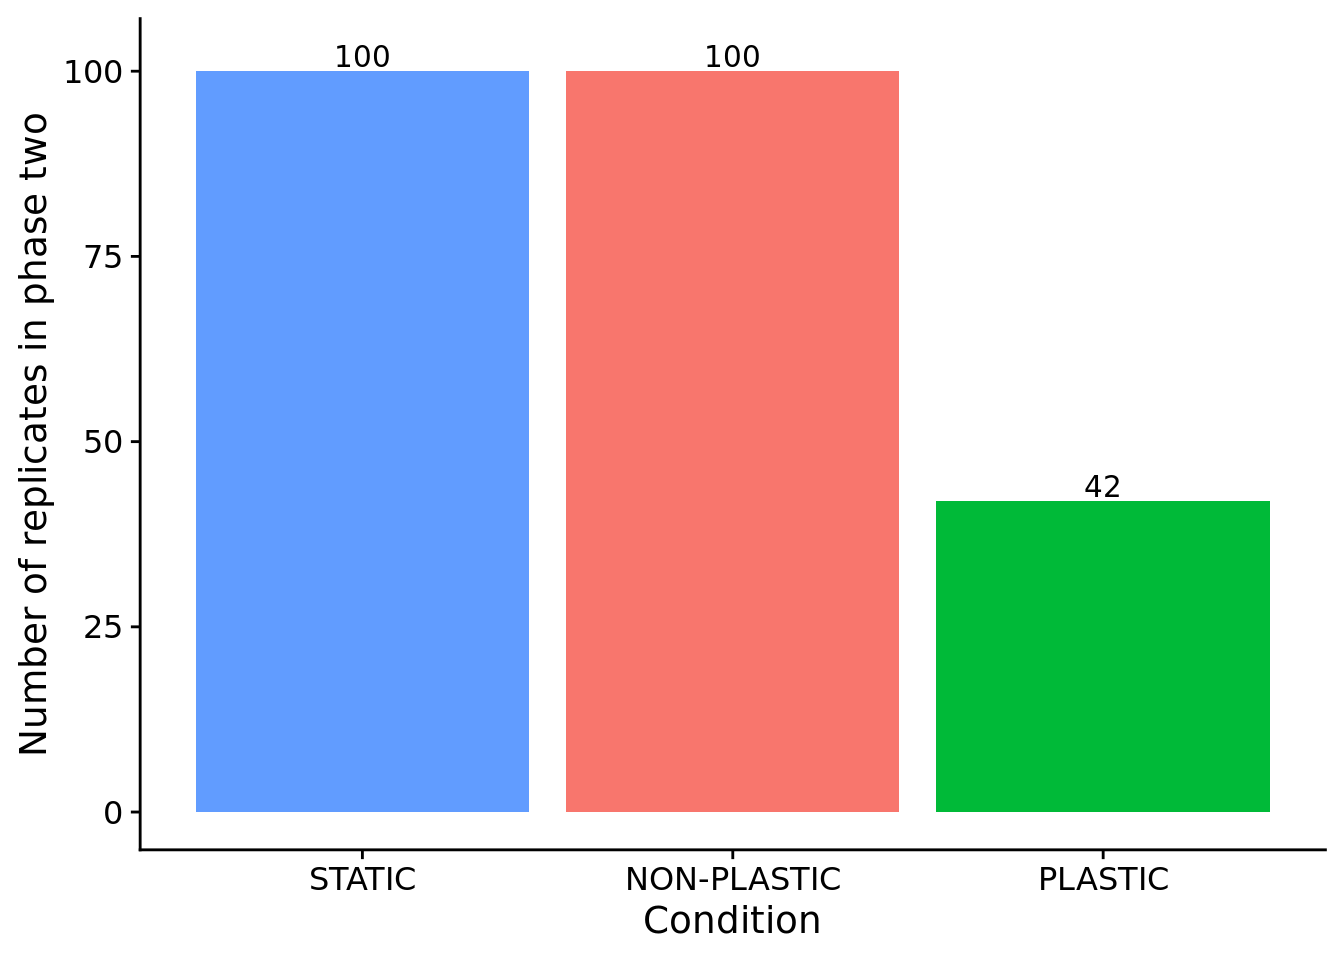
\includegraphics{supplemental-material_files/figure-latex/unnamed-chunk-11-1.pdf}

We can confirm our expectation that the dominant genotypes in non-plastic conditions are not phenotypically plastic.

\begin{Shaded}
\begin{Highlighting}[]
\NormalTok{summary_data_grouped =}\StringTok{ }\NormalTok{dplyr}\OperatorTok{::}\KeywordTok{group_by}\NormalTok{(summary_data, condition, is_plastic)}
\NormalTok{summary_data_group_counts =}\StringTok{ }\NormalTok{dplyr}\OperatorTok{::}\KeywordTok{summarize}\NormalTok{(summary_data_grouped, }\DataTypeTok{n=}\NormalTok{dplyr}\OperatorTok{::}\KeywordTok{n}\NormalTok{())}
\end{Highlighting}
\end{Shaded}

\begin{verbatim}
## `summarise()` has grouped output by 'condition'. You can override using the `.groups` argument.
\end{verbatim}

\begin{Shaded}
\begin{Highlighting}[]
\KeywordTok{ggplot}\NormalTok{(}\KeywordTok{filter}\NormalTok{(summary_data_group_counts, is_plastic), }\KeywordTok{aes}\NormalTok{(}\DataTypeTok{x=}\NormalTok{condition, }\DataTypeTok{y=}\NormalTok{n, }\DataTypeTok{fill=}\NormalTok{condition)) }\OperatorTok{+}
\StringTok{  }\KeywordTok{geom_col}\NormalTok{(}\DataTypeTok{position=}\KeywordTok{position_dodge}\NormalTok{(}\FloatTok{0.9}\NormalTok{)) }\OperatorTok{+}
\StringTok{  }\KeywordTok{scale_x_discrete}\NormalTok{(}
    \DataTypeTok{name=}\StringTok{"Condition"}\NormalTok{,}
    \DataTypeTok{limits=}\NormalTok{condition_order}
\NormalTok{  ) }\OperatorTok{+}
\StringTok{  }\KeywordTok{geom_text}\NormalTok{(}\KeywordTok{aes}\NormalTok{(}\DataTypeTok{label=}\NormalTok{n, }\DataTypeTok{y=}\NormalTok{n}\OperatorTok{+}\DecValTok{1}\NormalTok{)) }\OperatorTok{+}
\StringTok{  }\KeywordTok{ylab}\NormalTok{(}\StringTok{"Number of replicates with a plastic dominant genotype"}\NormalTok{) }\OperatorTok{+}
\StringTok{  }\KeywordTok{theme}\NormalTok{(}
    \DataTypeTok{legend.position=}\StringTok{"none"}
\NormalTok{  )}
\end{Highlighting}
\end{Shaded}

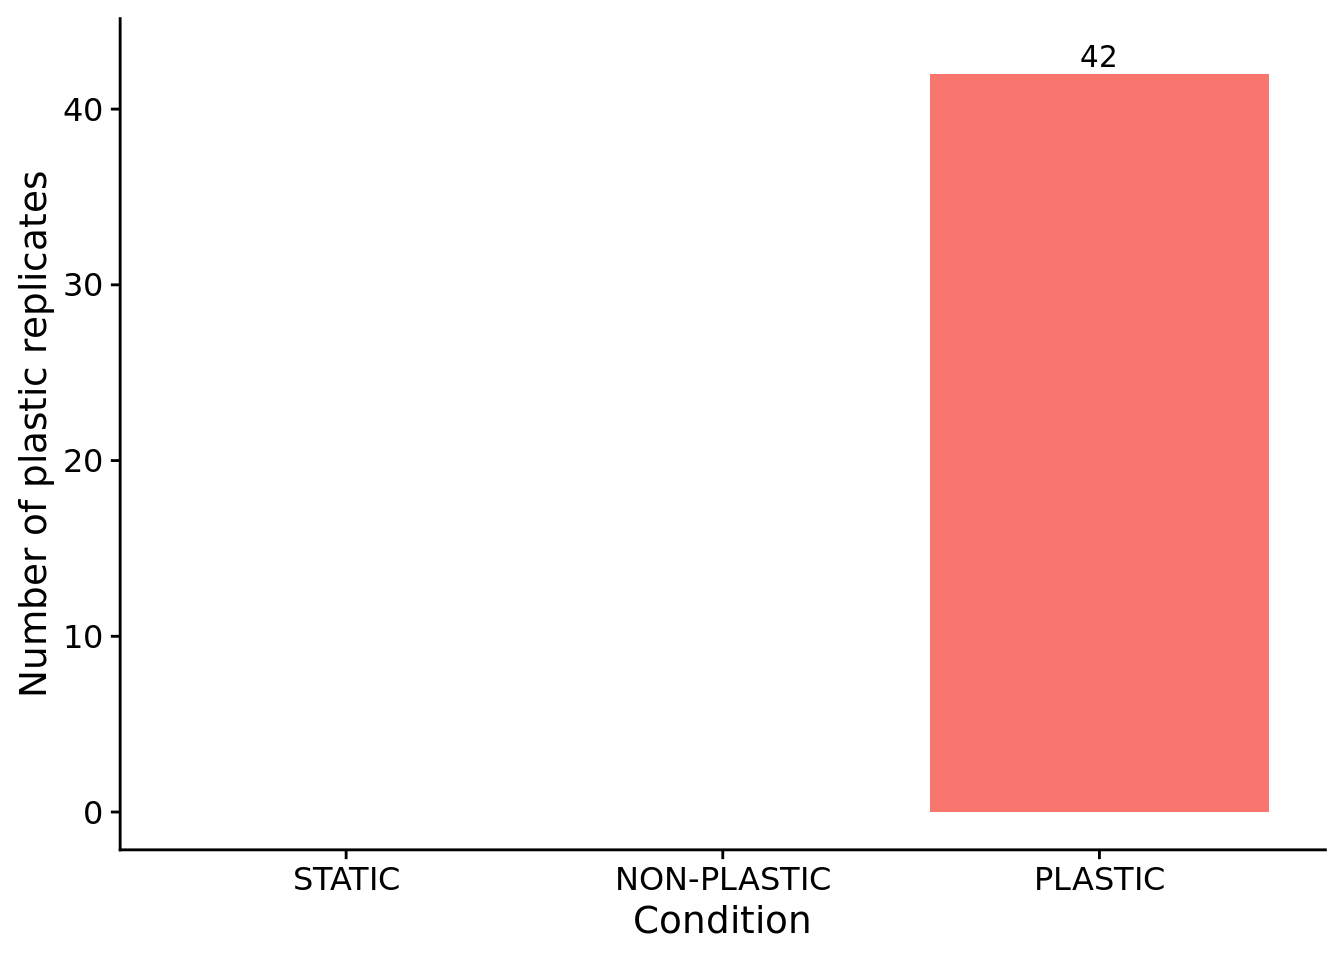
\includegraphics{supplemental-material_files/figure-latex/unnamed-chunk-12-1.pdf}

\hypertarget{phenotypic-volatility-along-dominant-lineage}{%
\section{Phenotypic volatility along dominant lineage}\label{phenotypic-volatility-along-dominant-lineage}}

\begin{Shaded}
\begin{Highlighting}[]
\KeywordTok{ggplot}\NormalTok{(summary_data, }\KeywordTok{aes}\NormalTok{(}\DataTypeTok{x=}\NormalTok{condition, }\DataTypeTok{y=}\NormalTok{dominant_lineage_phenotypic_volatility, }\DataTypeTok{fill=}\NormalTok{condition)) }\OperatorTok{+}
\StringTok{  }\KeywordTok{geom_flat_violin}\NormalTok{(}
    \DataTypeTok{position =} \KeywordTok{position_nudge}\NormalTok{(}\DataTypeTok{x =} \FloatTok{.2}\NormalTok{, }\DataTypeTok{y =} \DecValTok{0}\NormalTok{),}
    \DataTypeTok{alpha =} \FloatTok{.8}
\NormalTok{  ) }\OperatorTok{+}
\StringTok{  }\KeywordTok{geom_point}\NormalTok{(}
    \DataTypeTok{mapping=}\KeywordTok{aes}\NormalTok{(}\DataTypeTok{color=}\NormalTok{condition),}
    \DataTypeTok{position =} \KeywordTok{position_jitter}\NormalTok{(}\DataTypeTok{width =} \FloatTok{.15}\NormalTok{),}
    \DataTypeTok{size =} \FloatTok{.5}\NormalTok{,}
    \DataTypeTok{alpha =} \FloatTok{0.8}
\NormalTok{  ) }\OperatorTok{+}
\StringTok{  }\KeywordTok{geom_boxplot}\NormalTok{(}
    \DataTypeTok{width =} \FloatTok{.1}\NormalTok{,}
    \DataTypeTok{outlier.shape =} \OtherTok{NA}\NormalTok{,}
    \DataTypeTok{alpha =} \FloatTok{0.5}
\NormalTok{  ) }\OperatorTok{+}
\StringTok{  }\KeywordTok{scale_x_discrete}\NormalTok{(}
    \DataTypeTok{name=}\StringTok{"Condition"}\NormalTok{,}
    \DataTypeTok{limits=}\NormalTok{condition_order}
\NormalTok{  ) }\OperatorTok{+}
\StringTok{  }\KeywordTok{ylab}\NormalTok{(}\StringTok{"Phenotypic volatility"}\NormalTok{) }\OperatorTok{+}
\StringTok{  }\KeywordTok{theme}\NormalTok{(}
    \DataTypeTok{legend.position=}\StringTok{"none"}
\NormalTok{  )}
\end{Highlighting}
\end{Shaded}

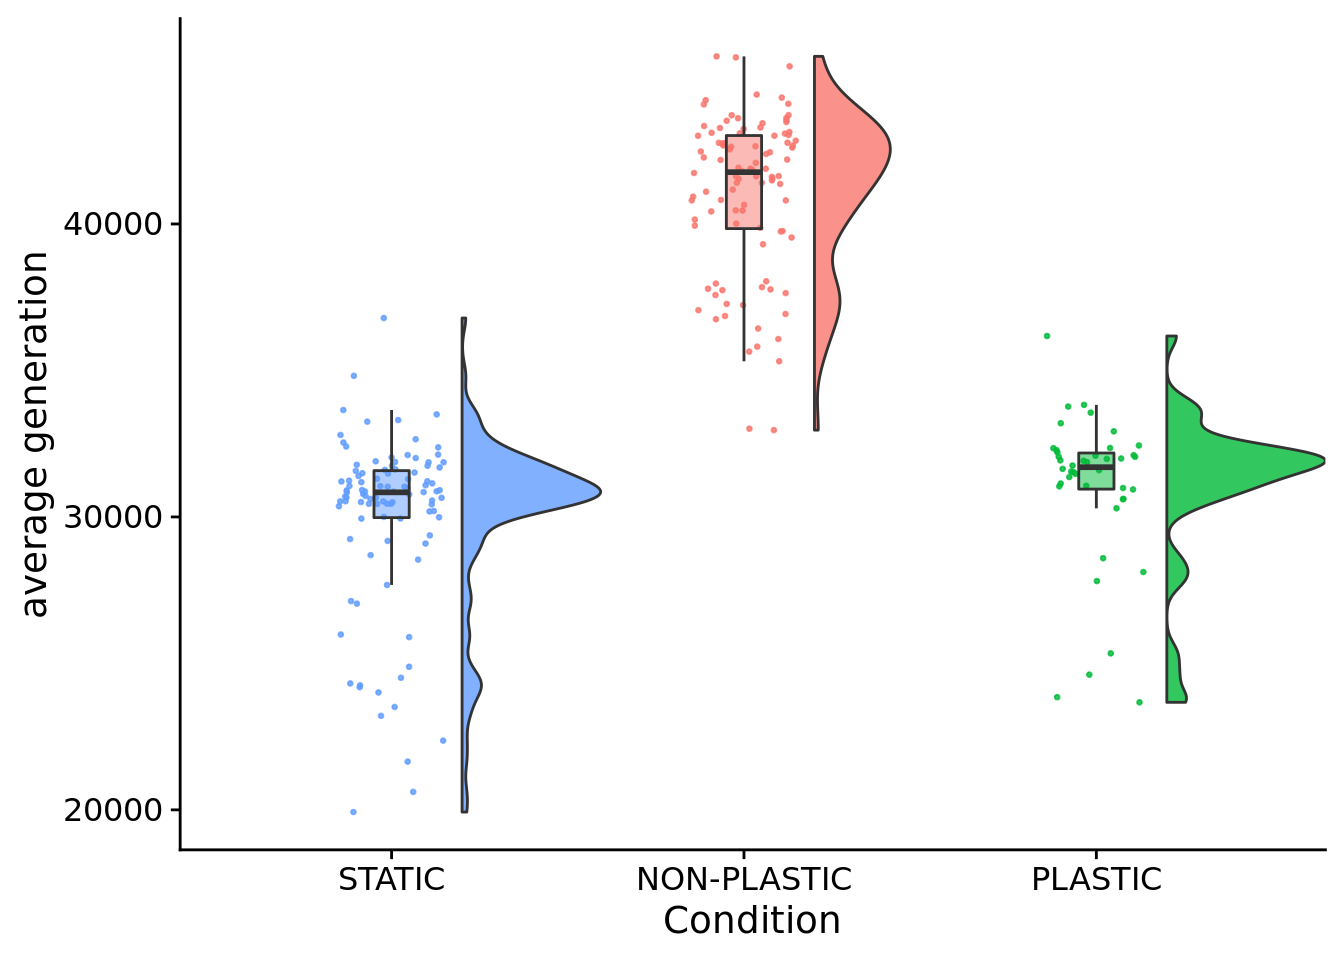
\includegraphics{supplemental-material_files/figure-latex/unnamed-chunk-13-1.pdf}

\begin{Shaded}
\begin{Highlighting}[]
\KeywordTok{kruskal.test}\NormalTok{(}
  \DataTypeTok{formula=}\NormalTok{dominant_lineage_phenotypic_volatility}\OperatorTok{~}\NormalTok{condition,}
  \DataTypeTok{data=}\NormalTok{summary_data}
\NormalTok{)}
\end{Highlighting}
\end{Shaded}

\begin{verbatim}
## 
##  Kruskal-Wallis rank sum test
## 
## data:  dominant_lineage_phenotypic_volatility by condition
## Kruskal-Wallis chi-squared = 351.93, df = 2, p-value < 2.2e-16
\end{verbatim}

\begin{Shaded}
\begin{Highlighting}[]
\KeywordTok{pairwise.wilcox.test}\NormalTok{(}
  \DataTypeTok{x=}\NormalTok{summary_data}\OperatorTok{$}\NormalTok{dominant_lineage_phenotypic_volatility,}
  \DataTypeTok{g=}\NormalTok{summary_data}\OperatorTok{$}\NormalTok{condition,}
  \DataTypeTok{p.adjust.method=}\StringTok{"bonferroni"}\NormalTok{,}
\NormalTok{)}
\end{Highlighting}
\end{Shaded}

\begin{verbatim}
## 
##  Pairwise comparisons using Wilcoxon rank sum test with continuity correction 
## 
## data:  summary_data$dominant_lineage_phenotypic_volatility and summary_data$condition 
## 
##                           Non-plastic (constant) Non-plastic (fluctuating)
## Non-plastic (fluctuating) <2e-16                 -                        
## Plastic (fluctuating)     0.014                  <2e-16                   
## 
## P value adjustment method: bonferroni
\end{verbatim}

\begin{Shaded}
\begin{Highlighting}[]
\KeywordTok{median}\NormalTok{(}\KeywordTok{filter}\NormalTok{(summary_data, condition}\OperatorTok{==}\StringTok{"Plastic (fluctuating)"}\NormalTok{)}\OperatorTok{$}\NormalTok{dominant_lineage_phenotypic_volatility)}
\end{Highlighting}
\end{Shaded}

\begin{verbatim}
## [1] 391
\end{verbatim}

\begin{Shaded}
\begin{Highlighting}[]
\KeywordTok{median}\NormalTok{(}\KeywordTok{filter}\NormalTok{(summary_data, condition}\OperatorTok{==}\StringTok{"Non-plastic (constant)"}\NormalTok{)}\OperatorTok{$}\NormalTok{dominant_lineage_phenotypic_volatility)}
\end{Highlighting}
\end{Shaded}

\begin{verbatim}
## [1] 356
\end{verbatim}

\begin{Shaded}
\begin{Highlighting}[]
\KeywordTok{median}\NormalTok{(}\KeywordTok{filter}\NormalTok{(summary_data, condition}\OperatorTok{==}\StringTok{"Non-plastic (fluctuating)"}\NormalTok{)}\OperatorTok{$}\NormalTok{dominant_lineage_phenotypic_volatility)}
\end{Highlighting}
\end{Shaded}

\begin{verbatim}
## [1] 1628
\end{verbatim}

\hypertarget{mutation-accumulation-along-dominant-lineage}{%
\section{Mutation accumulation along dominant lineage}\label{mutation-accumulation-along-dominant-lineage}}

\begin{Shaded}
\begin{Highlighting}[]
\KeywordTok{ggplot}\NormalTok{(summary_data, }\KeywordTok{aes}\NormalTok{(}\DataTypeTok{x=}\NormalTok{condition, }\DataTypeTok{y=}\NormalTok{dominant_lineage_total_mut_cnt, }\DataTypeTok{fill=}\NormalTok{condition)) }\OperatorTok{+}
\StringTok{  }\KeywordTok{geom_flat_violin}\NormalTok{(}
    \DataTypeTok{position =} \KeywordTok{position_nudge}\NormalTok{(}\DataTypeTok{x =} \FloatTok{.2}\NormalTok{, }\DataTypeTok{y =} \DecValTok{0}\NormalTok{),}
    \DataTypeTok{alpha =} \FloatTok{.8}
\NormalTok{  ) }\OperatorTok{+}
\StringTok{  }\KeywordTok{geom_point}\NormalTok{(}
    \DataTypeTok{mapping=}\KeywordTok{aes}\NormalTok{(}\DataTypeTok{color=}\NormalTok{condition),}
    \DataTypeTok{position =} \KeywordTok{position_jitter}\NormalTok{(}\DataTypeTok{width =} \FloatTok{.15}\NormalTok{),}
    \DataTypeTok{size =} \FloatTok{.5}\NormalTok{,}
    \DataTypeTok{alpha =} \FloatTok{0.8}
\NormalTok{  ) }\OperatorTok{+}
\StringTok{  }\KeywordTok{geom_boxplot}\NormalTok{(}
    \DataTypeTok{width =} \FloatTok{.1}\NormalTok{,}
    \DataTypeTok{outlier.shape =} \OtherTok{NA}\NormalTok{,}
    \DataTypeTok{alpha =} \FloatTok{0.5}
\NormalTok{  ) }\OperatorTok{+}
\StringTok{  }\KeywordTok{scale_x_discrete}\NormalTok{(}
    \DataTypeTok{name=}\StringTok{"Condition"}\NormalTok{,}
    \DataTypeTok{limits=}\NormalTok{condition_order}
\NormalTok{  ) }\OperatorTok{+}
\StringTok{  }\KeywordTok{ylab}\NormalTok{(}\StringTok{"Mutation accumulation"}\NormalTok{) }\OperatorTok{+}
\StringTok{  }\KeywordTok{theme}\NormalTok{(}
    \DataTypeTok{legend.position=}\StringTok{"none"}
\NormalTok{  )}
\end{Highlighting}
\end{Shaded}

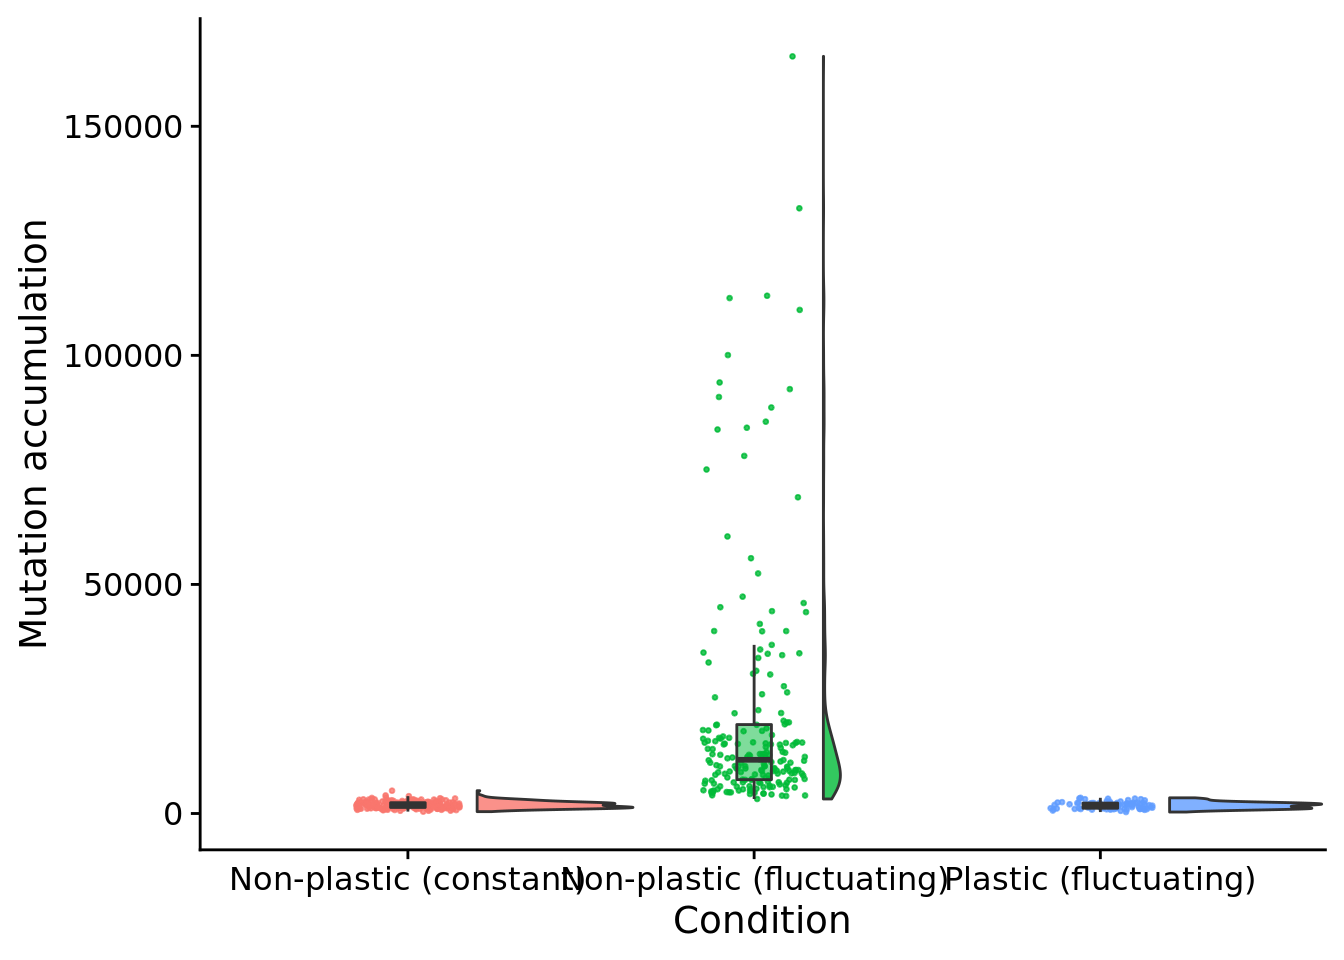
\includegraphics{supplemental-material_files/figure-latex/unnamed-chunk-15-1.pdf}

\begin{Shaded}
\begin{Highlighting}[]
\KeywordTok{kruskal.test}\NormalTok{(}
  \DataTypeTok{formula=}\NormalTok{dominant_lineage_total_mut_cnt}\OperatorTok{~}\NormalTok{condition,}
  \DataTypeTok{data=}\NormalTok{summary_data}
\NormalTok{)}
\end{Highlighting}
\end{Shaded}

\begin{verbatim}
## 
##  Kruskal-Wallis rank sum test
## 
## data:  dominant_lineage_total_mut_cnt by condition
## Kruskal-Wallis chi-squared = 352.67, df = 2, p-value < 2.2e-16
\end{verbatim}

\begin{Shaded}
\begin{Highlighting}[]
\KeywordTok{pairwise.wilcox.test}\NormalTok{(}
  \DataTypeTok{x=}\NormalTok{summary_data}\OperatorTok{$}\NormalTok{dominant_lineage_total_mut_cnt,}
  \DataTypeTok{g=}\NormalTok{summary_data}\OperatorTok{$}\NormalTok{condition,}
  \DataTypeTok{p.adjust.method=}\StringTok{"bonferroni"}\NormalTok{,}
\NormalTok{)}
\end{Highlighting}
\end{Shaded}

\begin{verbatim}
## 
##  Pairwise comparisons using Wilcoxon rank sum test with continuity correction 
## 
## data:  summary_data$dominant_lineage_total_mut_cnt and summary_data$condition 
## 
##                           Non-plastic (constant) Non-plastic (fluctuating)
## Non-plastic (fluctuating) <2e-16                 -                        
## Plastic (fluctuating)     0.65                   <2e-16                   
## 
## P value adjustment method: bonferroni
\end{verbatim}

\begin{Shaded}
\begin{Highlighting}[]
\KeywordTok{median}\NormalTok{(}\KeywordTok{filter}\NormalTok{(summary_data, condition}\OperatorTok{==}\StringTok{"Plastic (fluctuating)"}\NormalTok{)}\OperatorTok{$}\NormalTok{dominant_lineage_total_mut_cnt)}
\end{Highlighting}
\end{Shaded}

\begin{verbatim}
## [1] 1833
\end{verbatim}

\begin{Shaded}
\begin{Highlighting}[]
\KeywordTok{median}\NormalTok{(}\KeywordTok{filter}\NormalTok{(summary_data, condition}\OperatorTok{==}\StringTok{"Non-plastic (constant)"}\NormalTok{)}\OperatorTok{$}\NormalTok{dominant_lineage_total_mut_cnt)}
\end{Highlighting}
\end{Shaded}

\begin{verbatim}
## [1] 1823.5
\end{verbatim}

\begin{Shaded}
\begin{Highlighting}[]
\KeywordTok{median}\NormalTok{(}\KeywordTok{filter}\NormalTok{(summary_data, condition}\OperatorTok{==}\StringTok{"Non-plastic (fluctuating)"}\NormalTok{)}\OperatorTok{$}\NormalTok{dominant_lineage_total_mut_cnt)}
\end{Highlighting}
\end{Shaded}

\begin{verbatim}
## [1] 11721
\end{verbatim}

\hypertarget{mutation-accumulation-normalized-by-lineage-length}{%
\subsection{Mutation accumulation normalized by lineage length}\label{mutation-accumulation-normalized-by-lineage-length}}

\begin{Shaded}
\begin{Highlighting}[]
\NormalTok{summary_data}\OperatorTok{$}\NormalTok{mutations_per_lineage_step <-}\StringTok{ }\NormalTok{summary_data}\OperatorTok{$}\NormalTok{dominant_lineage_total_mut_cnt }\OperatorTok{/}\StringTok{ }\NormalTok{summary_data}\OperatorTok{$}\NormalTok{dominant_lineage_length_genotypes}
\KeywordTok{ggplot}\NormalTok{(summary_data, }\KeywordTok{aes}\NormalTok{(}\DataTypeTok{x=}\NormalTok{condition, }\DataTypeTok{y=}\NormalTok{mutations_per_lineage_step, }\DataTypeTok{fill=}\NormalTok{condition)) }\OperatorTok{+}
\StringTok{  }\KeywordTok{geom_flat_violin}\NormalTok{(}
    \DataTypeTok{position =} \KeywordTok{position_nudge}\NormalTok{(}\DataTypeTok{x =} \FloatTok{.2}\NormalTok{, }\DataTypeTok{y =} \DecValTok{0}\NormalTok{),}
    \DataTypeTok{alpha =} \FloatTok{.8}
\NormalTok{  ) }\OperatorTok{+}
\StringTok{  }\KeywordTok{geom_point}\NormalTok{(}
    \DataTypeTok{mapping=}\KeywordTok{aes}\NormalTok{(}\DataTypeTok{color=}\NormalTok{condition),}
    \DataTypeTok{position =} \KeywordTok{position_jitter}\NormalTok{(}\DataTypeTok{width =} \FloatTok{.15}\NormalTok{),}
    \DataTypeTok{size =} \FloatTok{.5}\NormalTok{,}
    \DataTypeTok{alpha =} \FloatTok{0.8}
\NormalTok{  ) }\OperatorTok{+}
\StringTok{  }\KeywordTok{geom_boxplot}\NormalTok{(}
    \DataTypeTok{width =} \FloatTok{.1}\NormalTok{,}
    \DataTypeTok{outlier.shape =} \OtherTok{NA}\NormalTok{,}
    \DataTypeTok{alpha =} \FloatTok{0.5}
\NormalTok{  ) }\OperatorTok{+}
\StringTok{  }\KeywordTok{scale_x_discrete}\NormalTok{(}
    \DataTypeTok{name=}\StringTok{"Condition"}\NormalTok{,}
    \DataTypeTok{limits=}\NormalTok{condition_order}
\NormalTok{  ) }\OperatorTok{+}
\StringTok{  }\KeywordTok{ylab}\NormalTok{(}\StringTok{"Mutation accumulation / lineage length"}\NormalTok{) }\OperatorTok{+}
\StringTok{  }\KeywordTok{theme}\NormalTok{(}
    \DataTypeTok{legend.position=}\StringTok{"none"}
\NormalTok{  )}
\end{Highlighting}
\end{Shaded}

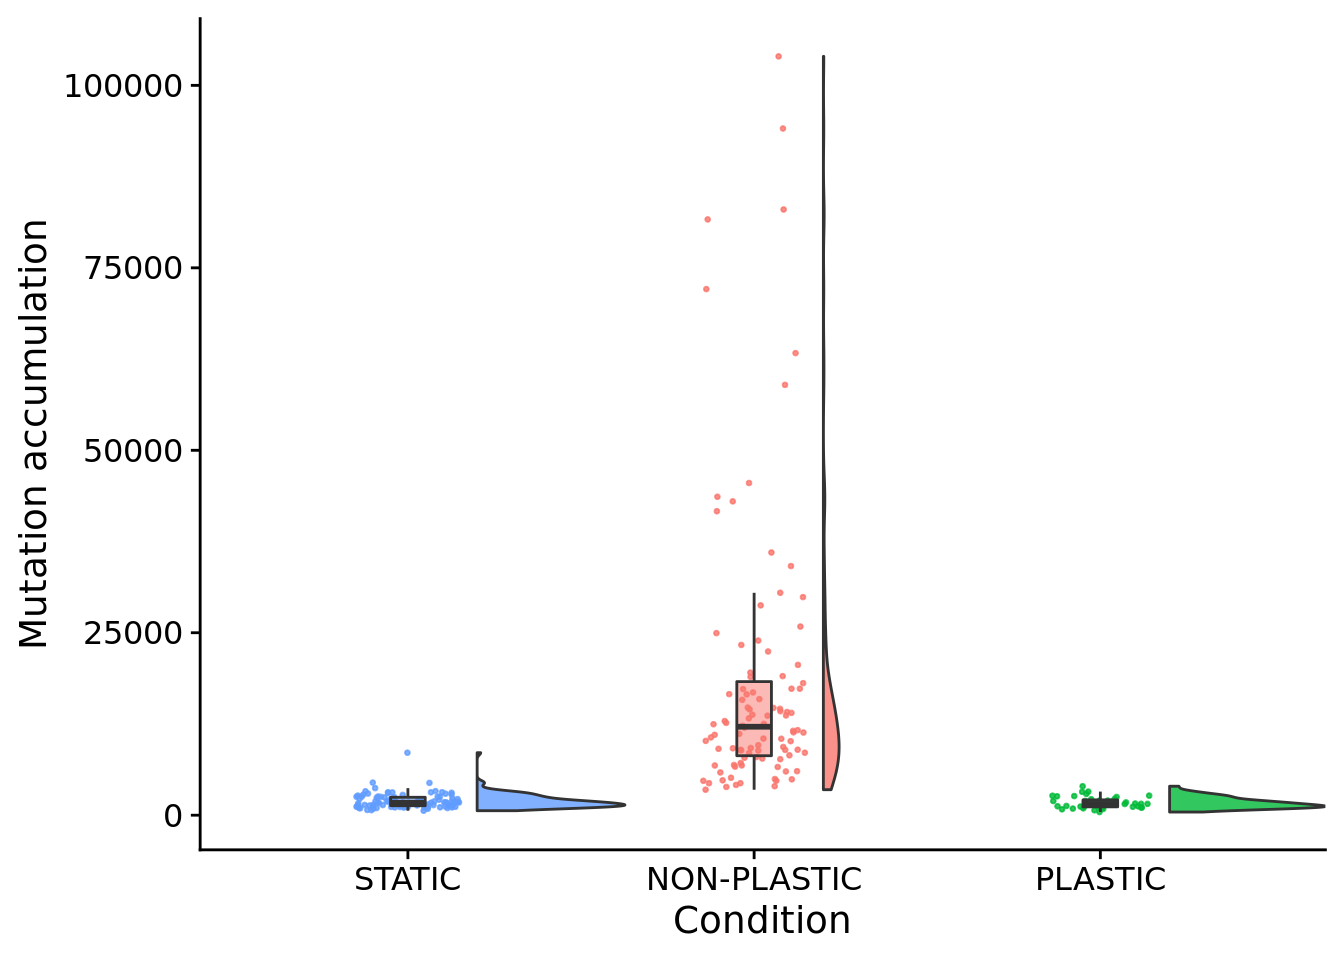
\includegraphics{supplemental-material_files/figure-latex/unnamed-chunk-17-1.pdf}

\begin{Shaded}
\begin{Highlighting}[]
\KeywordTok{kruskal.test}\NormalTok{(}
  \DataTypeTok{formula=}\NormalTok{mutations_per_lineage_step}\OperatorTok{~}\NormalTok{condition,}
  \DataTypeTok{data=}\NormalTok{summary_data}
\NormalTok{)}
\end{Highlighting}
\end{Shaded}

\begin{verbatim}
## 
##  Kruskal-Wallis rank sum test
## 
## data:  mutations_per_lineage_step by condition
## Kruskal-Wallis chi-squared = 194.32, df = 2, p-value < 2.2e-16
\end{verbatim}

\begin{Shaded}
\begin{Highlighting}[]
\KeywordTok{pairwise.wilcox.test}\NormalTok{(}
  \DataTypeTok{x=}\NormalTok{summary_data}\OperatorTok{$}\NormalTok{mutations_per_lineage_step,}
  \DataTypeTok{g=}\NormalTok{summary_data}\OperatorTok{$}\NormalTok{condition,}
  \DataTypeTok{p.adjust.method=}\StringTok{"bonferroni"}\NormalTok{,}
\NormalTok{)}
\end{Highlighting}
\end{Shaded}

\begin{verbatim}
## 
##  Pairwise comparisons using Wilcoxon rank sum test with continuity correction 
## 
## data:  summary_data$mutations_per_lineage_step and summary_data$condition 
## 
##                           Non-plastic (constant) Non-plastic (fluctuating)
## Non-plastic (fluctuating) <2e-16                 -                        
## Plastic (fluctuating)     1                      <2e-16                   
## 
## P value adjustment method: bonferroni
\end{verbatim}

\begin{Shaded}
\begin{Highlighting}[]
\KeywordTok{median}\NormalTok{(}\KeywordTok{filter}\NormalTok{(summary_data, condition}\OperatorTok{==}\StringTok{"Plastic (fluctuating)"}\NormalTok{)}\OperatorTok{$}\NormalTok{mutations_per_lineage_step)}
\end{Highlighting}
\end{Shaded}

\begin{verbatim}
## [1] 1.504491
\end{verbatim}

\begin{Shaded}
\begin{Highlighting}[]
\KeywordTok{median}\NormalTok{(}\KeywordTok{filter}\NormalTok{(summary_data, condition}\OperatorTok{==}\StringTok{"Non-plastic (constant)"}\NormalTok{)}\OperatorTok{$}\NormalTok{mutations_per_lineage_step)}
\end{Highlighting}
\end{Shaded}

\begin{verbatim}
## [1] 1.526001
\end{verbatim}

\begin{Shaded}
\begin{Highlighting}[]
\KeywordTok{median}\NormalTok{(}\KeywordTok{filter}\NormalTok{(summary_data, condition}\OperatorTok{==}\StringTok{"Non-plastic (fluctuating)"}\NormalTok{)}\OperatorTok{$}\NormalTok{mutations_per_lineage_step)}
\end{Highlighting}
\end{Shaded}

\begin{verbatim}
## [1] 2.645598
\end{verbatim}

\hypertarget{selective-sweeps}{%
\section{Selective sweeps}\label{selective-sweeps}}

The number of times the most recent common ancestor changes gives us the number of selective sweeps that occur during the experiment.

\begin{Shaded}
\begin{Highlighting}[]
\KeywordTok{ggplot}\NormalTok{(summary_data, }\KeywordTok{aes}\NormalTok{(}\DataTypeTok{x=}\NormalTok{condition, }\DataTypeTok{y=}\NormalTok{phylo_mrca_changes, }\DataTypeTok{fill=}\NormalTok{condition)) }\OperatorTok{+}
\StringTok{  }\KeywordTok{geom_flat_violin}\NormalTok{(}
    \DataTypeTok{position =} \KeywordTok{position_nudge}\NormalTok{(}\DataTypeTok{x =} \FloatTok{.2}\NormalTok{, }\DataTypeTok{y =} \DecValTok{0}\NormalTok{),}
    \DataTypeTok{alpha =} \FloatTok{.8}
\NormalTok{  ) }\OperatorTok{+}
\StringTok{  }\KeywordTok{geom_point}\NormalTok{(}
    \DataTypeTok{mapping=}\KeywordTok{aes}\NormalTok{(}\DataTypeTok{color=}\NormalTok{condition),}
    \DataTypeTok{position =} \KeywordTok{position_jitter}\NormalTok{(}\DataTypeTok{width =} \FloatTok{.15}\NormalTok{),}
    \DataTypeTok{size =} \FloatTok{.5}\NormalTok{,}
    \DataTypeTok{alpha =} \FloatTok{0.8}
\NormalTok{  ) }\OperatorTok{+}
\StringTok{  }\KeywordTok{geom_boxplot}\NormalTok{(}
    \DataTypeTok{width =} \FloatTok{.1}\NormalTok{,}
    \DataTypeTok{outlier.shape =} \OtherTok{NA}\NormalTok{,}
    \DataTypeTok{alpha =} \FloatTok{0.5}
\NormalTok{  ) }\OperatorTok{+}
\StringTok{  }\KeywordTok{scale_x_discrete}\NormalTok{(}
    \DataTypeTok{name=}\StringTok{"Condition"}\NormalTok{,}
    \DataTypeTok{limits=}\NormalTok{condition_order}
\NormalTok{  ) }\OperatorTok{+}
\StringTok{  }\KeywordTok{ylab}\NormalTok{(}\StringTok{"Number of selective sweeps"}\NormalTok{) }\OperatorTok{+}
\StringTok{  }\KeywordTok{theme}\NormalTok{(}
    \DataTypeTok{legend.position=}\StringTok{"none"}
\NormalTok{  )}
\end{Highlighting}
\end{Shaded}

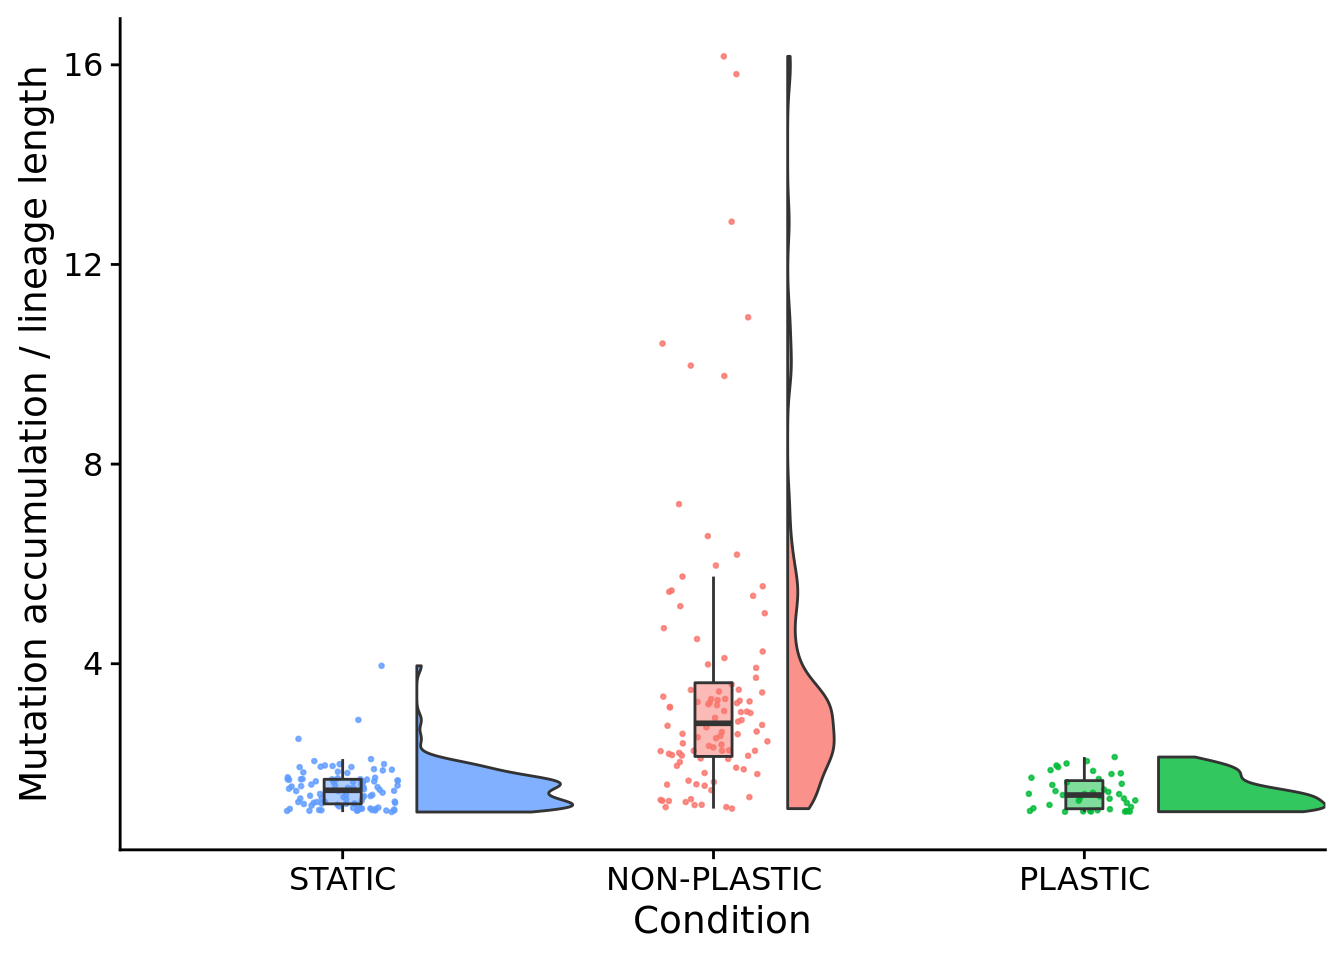
\includegraphics{supplemental-material_files/figure-latex/unnamed-chunk-19-1.pdf}

\begin{Shaded}
\begin{Highlighting}[]
\KeywordTok{kruskal.test}\NormalTok{(}
  \DataTypeTok{formula=}\NormalTok{phylo_mrca_changes}\OperatorTok{~}\NormalTok{condition,}
  \DataTypeTok{data=}\NormalTok{summary_data}
\NormalTok{)}
\end{Highlighting}
\end{Shaded}

\begin{verbatim}
## 
##  Kruskal-Wallis rank sum test
## 
## data:  phylo_mrca_changes by condition
## Kruskal-Wallis chi-squared = 182.92, df = 2, p-value < 2.2e-16
\end{verbatim}

\begin{Shaded}
\begin{Highlighting}[]
\KeywordTok{pairwise.wilcox.test}\NormalTok{(}
  \DataTypeTok{x=}\NormalTok{summary_data}\OperatorTok{$}\NormalTok{phylo_mrca_changes,}
  \DataTypeTok{g=}\NormalTok{summary_data}\OperatorTok{$}\NormalTok{condition,}
  \DataTypeTok{p.adjust.method=}\StringTok{"bonferroni"}\NormalTok{,}
\NormalTok{)}
\end{Highlighting}
\end{Shaded}

\begin{verbatim}
## 
##  Pairwise comparisons using Wilcoxon rank sum test with continuity correction 
## 
## data:  summary_data$phylo_mrca_changes and summary_data$condition 
## 
##                           Non-plastic (constant) Non-plastic (fluctuating)
## Non-plastic (fluctuating) <2e-16                 -                        
## Plastic (fluctuating)     0.35                   <2e-16                   
## 
## P value adjustment method: bonferroni
\end{verbatim}

\begin{Shaded}
\begin{Highlighting}[]
\KeywordTok{median}\NormalTok{(}\KeywordTok{filter}\NormalTok{(summary_data, condition}\OperatorTok{==}\StringTok{"Plastic (fluctuating)"}\NormalTok{)}\OperatorTok{$}\NormalTok{phylo_mrca_changes)}
\end{Highlighting}
\end{Shaded}

\begin{verbatim}
## [1] 49
\end{verbatim}

\begin{Shaded}
\begin{Highlighting}[]
\KeywordTok{median}\NormalTok{(}\KeywordTok{filter}\NormalTok{(summary_data, condition}\OperatorTok{==}\StringTok{"Non-plastic (constant)"}\NormalTok{)}\OperatorTok{$}\NormalTok{phylo_mrca_changes)}
\end{Highlighting}
\end{Shaded}

\begin{verbatim}
## [1] 47
\end{verbatim}

\begin{Shaded}
\begin{Highlighting}[]
\KeywordTok{median}\NormalTok{(}\KeywordTok{filter}\NormalTok{(summary_data, condition}\OperatorTok{==}\StringTok{"Non-plastic (fluctuating)"}\NormalTok{)}\OperatorTok{$}\NormalTok{phylo_mrca_changes)}
\end{Highlighting}
\end{Shaded}

\begin{verbatim}
## [1] 288.5
\end{verbatim}

\hypertarget{genome-length}{%
\section{Genome length}\label{genome-length}}

\begin{Shaded}
\begin{Highlighting}[]
\KeywordTok{ggplot}\NormalTok{(summary_data, }\KeywordTok{aes}\NormalTok{(}\DataTypeTok{x=}\NormalTok{condition, }\DataTypeTok{y=}\NormalTok{dominant_genome_length, }\DataTypeTok{fill=}\NormalTok{condition)) }\OperatorTok{+}
\StringTok{  }\KeywordTok{geom_flat_violin}\NormalTok{(}
    \DataTypeTok{position =} \KeywordTok{position_nudge}\NormalTok{(}\DataTypeTok{x =} \FloatTok{.2}\NormalTok{, }\DataTypeTok{y =} \DecValTok{0}\NormalTok{),}
    \DataTypeTok{alpha =} \FloatTok{.8}
\NormalTok{  ) }\OperatorTok{+}
\StringTok{  }\KeywordTok{geom_point}\NormalTok{(}
    \DataTypeTok{mapping=}\KeywordTok{aes}\NormalTok{(}\DataTypeTok{color=}\NormalTok{condition),}
    \DataTypeTok{position =} \KeywordTok{position_jitter}\NormalTok{(}\DataTypeTok{width =} \FloatTok{.15}\NormalTok{),}
    \DataTypeTok{size =} \FloatTok{.5}\NormalTok{,}
    \DataTypeTok{alpha =} \FloatTok{0.8}
\NormalTok{  ) }\OperatorTok{+}
\StringTok{  }\KeywordTok{geom_boxplot}\NormalTok{(}
    \DataTypeTok{width =} \FloatTok{.1}\NormalTok{,}
    \DataTypeTok{outlier.shape =} \OtherTok{NA}\NormalTok{,}
    \DataTypeTok{alpha =} \FloatTok{0.5}
\NormalTok{  ) }\OperatorTok{+}
\StringTok{  }\KeywordTok{scale_x_discrete}\NormalTok{(}
    \DataTypeTok{name=}\StringTok{"Condition"}\NormalTok{,}
    \DataTypeTok{limits=}\NormalTok{condition_order}
\NormalTok{  ) }\OperatorTok{+}
\StringTok{  }\KeywordTok{ylab}\NormalTok{(}\StringTok{"Genome length"}\NormalTok{) }\OperatorTok{+}
\StringTok{  }\KeywordTok{theme}\NormalTok{(}
    \DataTypeTok{legend.position=}\StringTok{"none"}
\NormalTok{  )}
\end{Highlighting}
\end{Shaded}

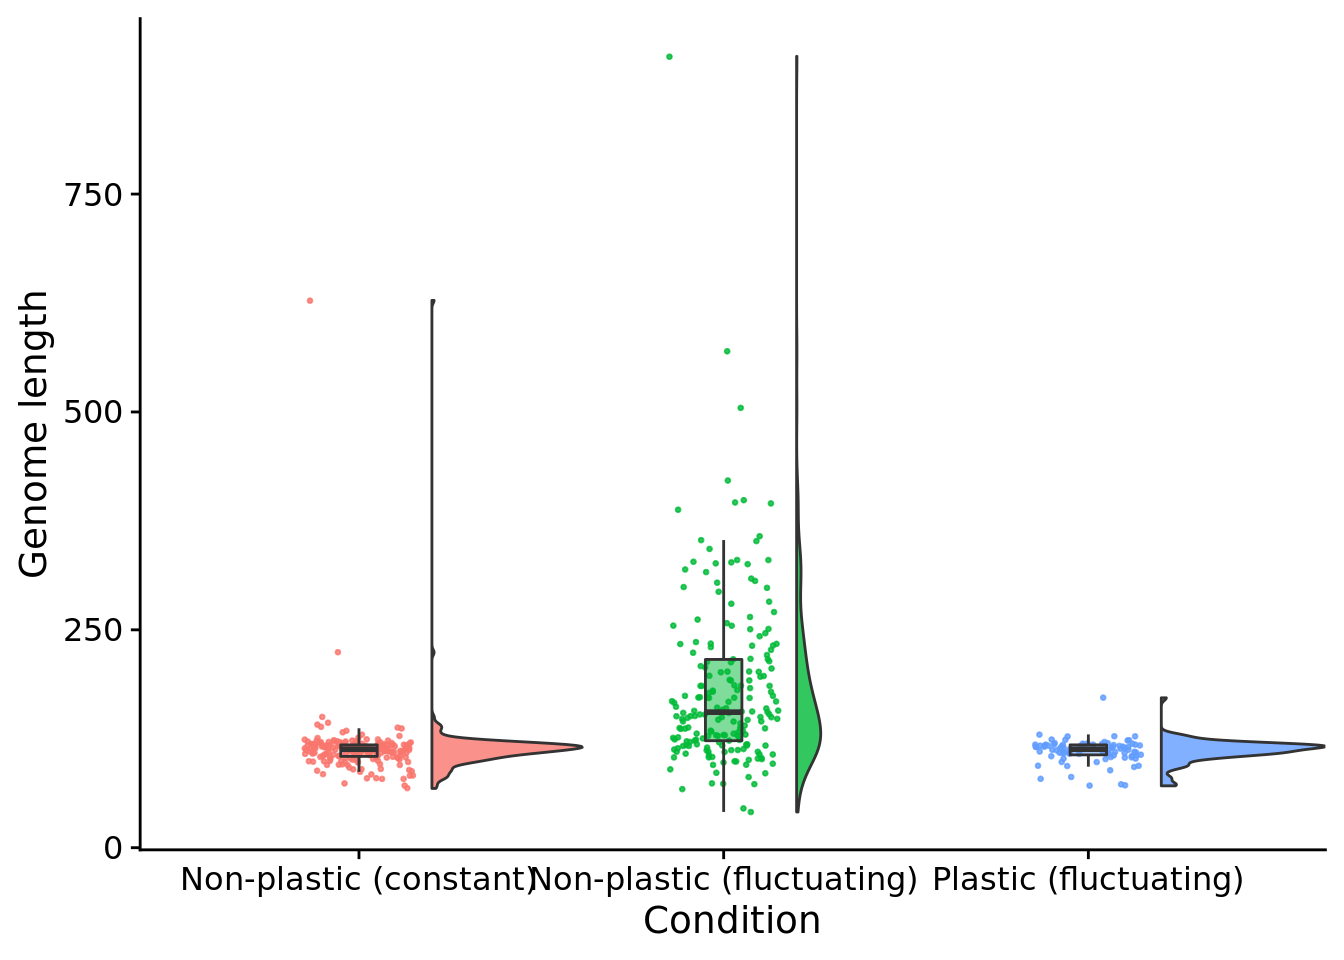
\includegraphics{supplemental-material_files/figure-latex/unnamed-chunk-21-1.pdf}

\hypertarget{diversity-over-time}{%
\section{Diversity over time}\label{diversity-over-time}}

\hypertarget{shannon-entropy-over-time}{%
\subsection{Shannon entropy over time}\label{shannon-entropy-over-time}}

\begin{Shaded}
\begin{Highlighting}[]
\CommentTok{# shannon entropy}
\KeywordTok{ggplot}\NormalTok{(time_series_data, }\KeywordTok{aes}\NormalTok{(}\DataTypeTok{x=}\NormalTok{update, }\DataTypeTok{y=}\NormalTok{phylo_diversity, }\DataTypeTok{fill=}\NormalTok{condition, }\DataTypeTok{color=}\NormalTok{condition)) }\OperatorTok{+}
\StringTok{  }\KeywordTok{stat_summary}\NormalTok{(}\DataTypeTok{fun=}\StringTok{"mean"}\NormalTok{, }\DataTypeTok{geom=}\StringTok{"line"}\NormalTok{) }\OperatorTok{+}
\StringTok{  }\KeywordTok{stat_summary}\NormalTok{(}
    \DataTypeTok{fun.data=}\StringTok{"mean_cl_boot"}\NormalTok{,}
    \DataTypeTok{fun.args=}\KeywordTok{list}\NormalTok{(}\DataTypeTok{conf.int=}\FloatTok{0.95}\NormalTok{),}
    \DataTypeTok{geom=}\StringTok{"ribbon"}\NormalTok{,}
    \DataTypeTok{alpha=}\FloatTok{0.2}\NormalTok{,}
    \DataTypeTok{linetype=}\DecValTok{0}
\NormalTok{  ) }\OperatorTok{+}
\StringTok{  }\KeywordTok{ylab}\NormalTok{(}\StringTok{"Shannon entropy"}\NormalTok{)}
\end{Highlighting}
\end{Shaded}

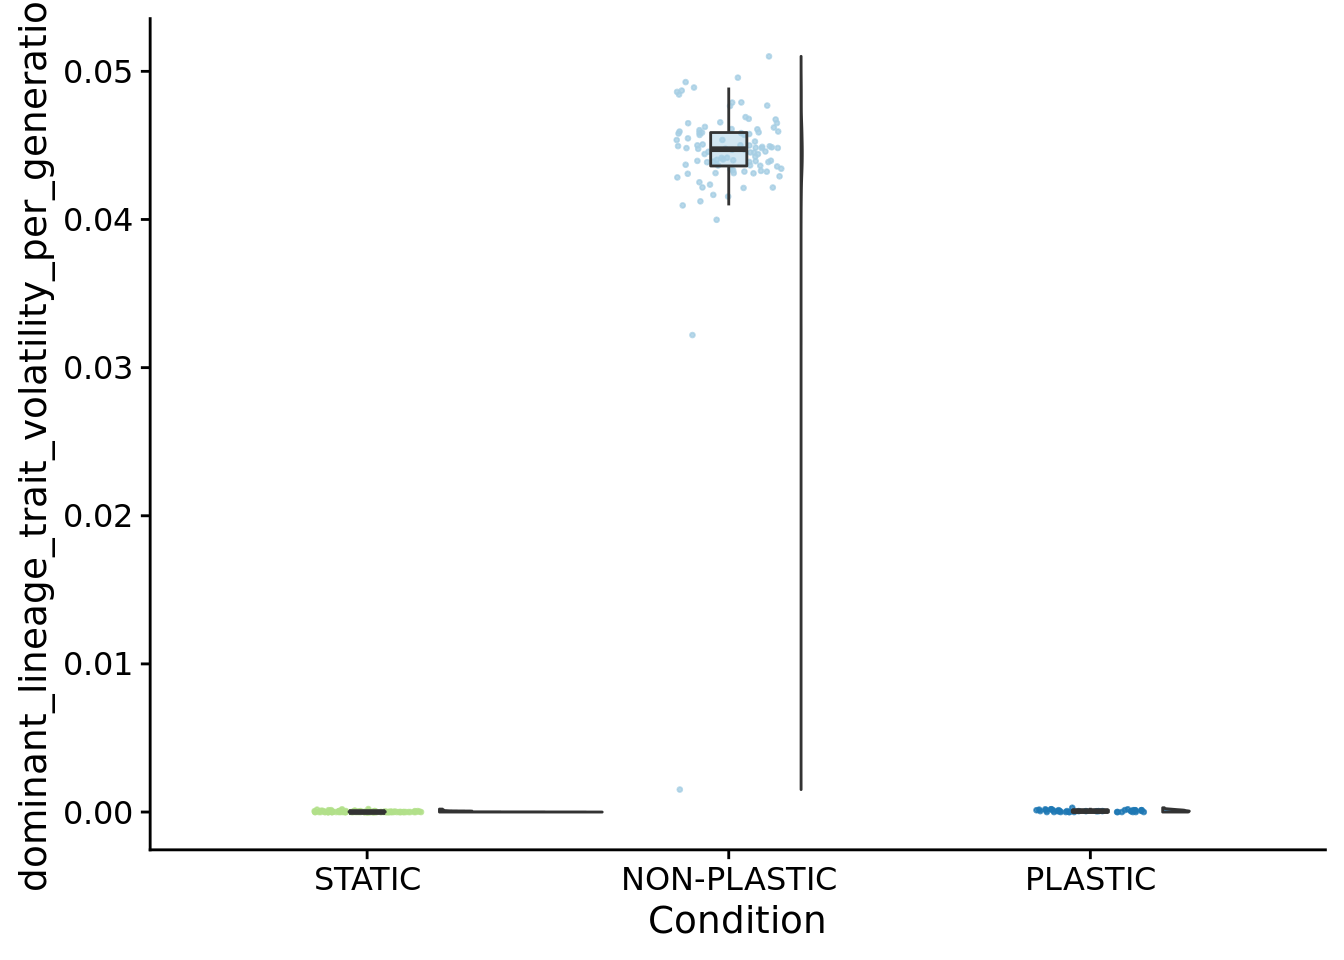
\includegraphics{supplemental-material_files/figure-latex/unnamed-chunk-22-1.pdf}

Zoom in to just 400 update span.

\begin{Shaded}
\begin{Highlighting}[]
\CommentTok{# shannon entropy}
\KeywordTok{ggplot}\NormalTok{(}\KeywordTok{filter}\NormalTok{(time_series_data, update }\OperatorTok{<=}\StringTok{ }\DecValTok{10400}\NormalTok{), }\KeywordTok{aes}\NormalTok{(}\DataTypeTok{x=}\NormalTok{update, }\DataTypeTok{y=}\NormalTok{phylo_diversity, }\DataTypeTok{fill=}\NormalTok{condition, }\DataTypeTok{color=}\NormalTok{condition)) }\OperatorTok{+}
\StringTok{  }\KeywordTok{stat_summary}\NormalTok{(}\DataTypeTok{fun=}\StringTok{"mean"}\NormalTok{, }\DataTypeTok{geom=}\StringTok{"line"}\NormalTok{) }\OperatorTok{+}
\StringTok{  }\KeywordTok{stat_summary}\NormalTok{(}
    \DataTypeTok{fun.data=}\StringTok{"mean_cl_boot"}\NormalTok{,}
    \DataTypeTok{fun.args=}\KeywordTok{list}\NormalTok{(}\DataTypeTok{conf.int=}\FloatTok{0.95}\NormalTok{),}
    \DataTypeTok{geom=}\StringTok{"ribbon"}\NormalTok{,}
    \DataTypeTok{alpha=}\FloatTok{0.2}\NormalTok{,}
    \DataTypeTok{linetype=}\DecValTok{0}
\NormalTok{  ) }\OperatorTok{+}
\StringTok{  }\KeywordTok{ylab}\NormalTok{(}\StringTok{"Shannon entropy"}\NormalTok{)}
\end{Highlighting}
\end{Shaded}

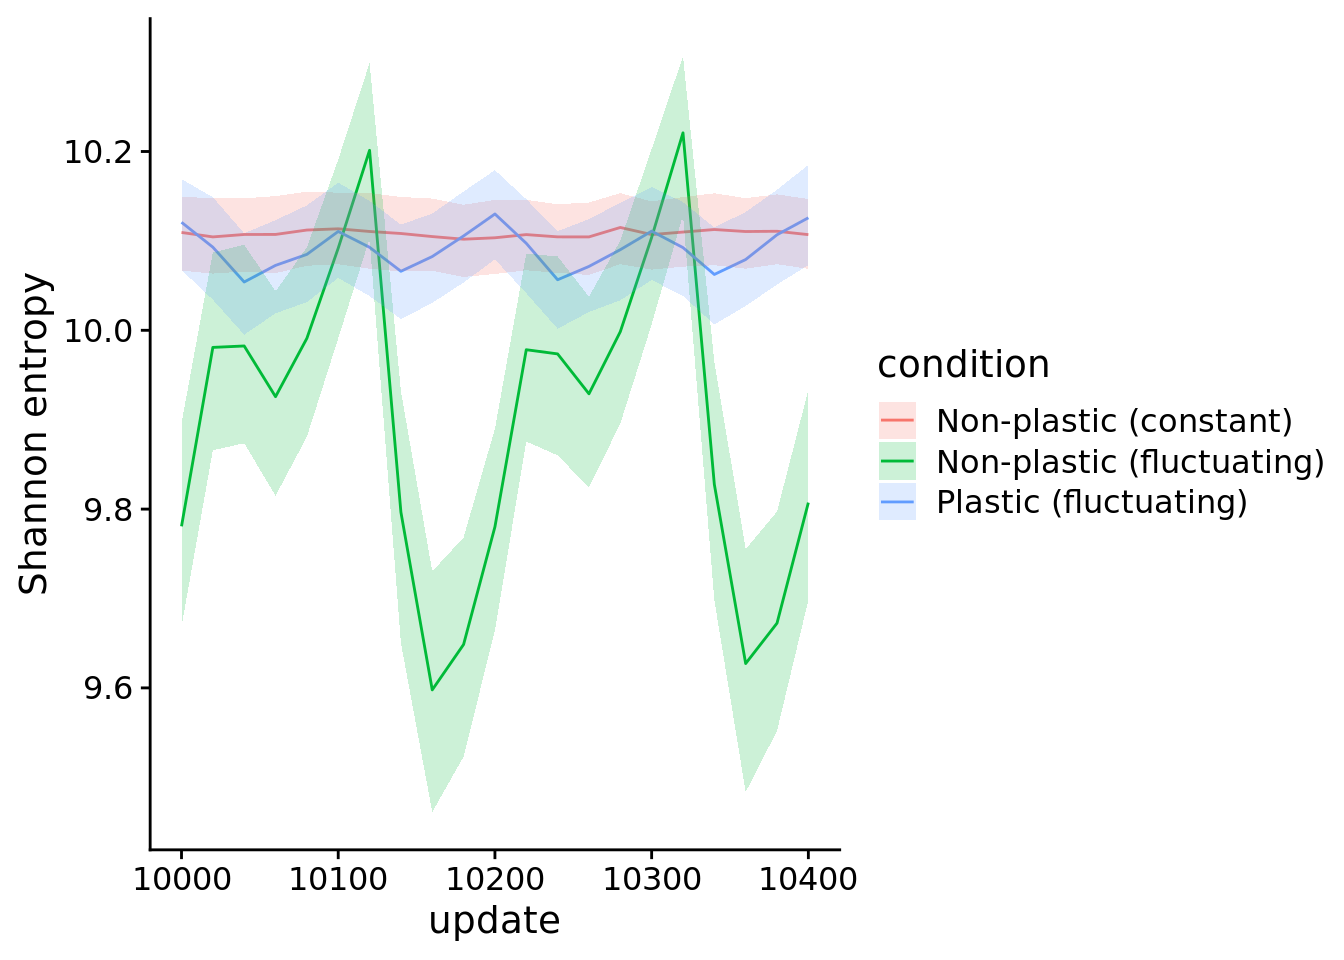
\includegraphics{supplemental-material_files/figure-latex/unnamed-chunk-23-1.pdf}

\hypertarget{phylogenetic-diversity-over-time}{%
\subsection{Phylogenetic diversity over time}\label{phylogenetic-diversity-over-time}}

\begin{verbatim}
// From (Faith 1992, reviewed in Winters et al., 2013), phylogenetic diversity is the sum of edges in the minimal spanning tree connected the taxa you're calculating diversity of.
// This calculates phylogenetic diversity for all extant taxa in the tree.
\end{verbatim}

\begin{Shaded}
\begin{Highlighting}[]
\KeywordTok{ggplot}\NormalTok{(time_series_data, }\KeywordTok{aes}\NormalTok{(}\DataTypeTok{x=}\NormalTok{update, }\DataTypeTok{y=}\NormalTok{phylo_current_phylogenetic_diversity, }\DataTypeTok{fill=}\NormalTok{condition, }\DataTypeTok{color=}\NormalTok{condition)) }\OperatorTok{+}
\StringTok{  }\KeywordTok{stat_summary}\NormalTok{(}\DataTypeTok{fun=}\StringTok{"mean"}\NormalTok{, }\DataTypeTok{geom=}\StringTok{"line"}\NormalTok{) }\OperatorTok{+}
\StringTok{  }\KeywordTok{stat_summary}\NormalTok{(}
    \DataTypeTok{fun.data=}\StringTok{"mean_cl_boot"}\NormalTok{,}
    \DataTypeTok{fun.args=}\KeywordTok{list}\NormalTok{(}\DataTypeTok{conf.int=}\FloatTok{0.95}\NormalTok{),}
    \DataTypeTok{geom=}\StringTok{"ribbon"}\NormalTok{,}
    \DataTypeTok{alpha=}\FloatTok{0.2}\NormalTok{,}
    \DataTypeTok{linetype=}\DecValTok{0}
\NormalTok{  ) }\OperatorTok{+}
\StringTok{  }\KeywordTok{ylab}\NormalTok{(}\StringTok{"Phylogenetic diversity"}\NormalTok{)}
\end{Highlighting}
\end{Shaded}

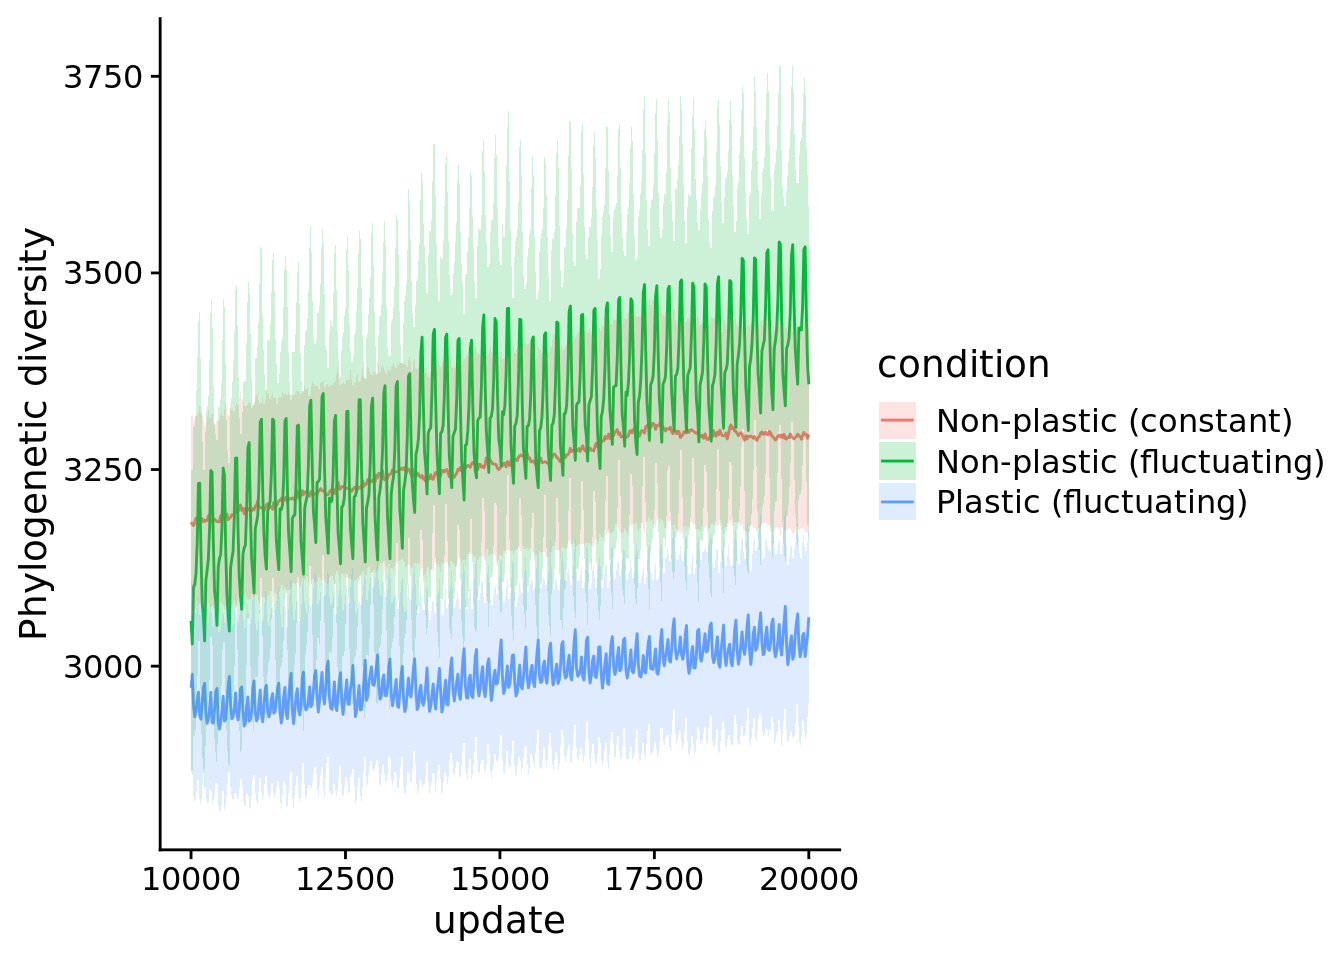
\includegraphics{supplemental-material_files/figure-latex/unnamed-chunk-24-1.pdf}

\hypertarget{number-of-extant-taxa-genotypes-over-time}{%
\subsection{Number of extant taxa (genotypes) over time}\label{number-of-extant-taxa-genotypes-over-time}}

\begin{Shaded}
\begin{Highlighting}[]
\KeywordTok{ggplot}\NormalTok{(time_series_data, }\KeywordTok{aes}\NormalTok{(}\DataTypeTok{x=}\NormalTok{update, }\DataTypeTok{y=}\NormalTok{phylo_num_taxa_extant, }\DataTypeTok{fill=}\NormalTok{condition, }\DataTypeTok{color=}\NormalTok{condition)) }\OperatorTok{+}
\StringTok{  }\KeywordTok{stat_summary}\NormalTok{(}\DataTypeTok{fun=}\StringTok{"mean"}\NormalTok{, }\DataTypeTok{geom=}\StringTok{"line"}\NormalTok{) }\OperatorTok{+}
\StringTok{  }\KeywordTok{stat_summary}\NormalTok{(}
    \DataTypeTok{fun.data=}\StringTok{"mean_cl_boot"}\NormalTok{,}
    \DataTypeTok{fun.args=}\KeywordTok{list}\NormalTok{(}\DataTypeTok{conf.int=}\FloatTok{0.95}\NormalTok{),}
    \DataTypeTok{geom=}\StringTok{"ribbon"}\NormalTok{,}
    \DataTypeTok{alpha=}\FloatTok{0.2}\NormalTok{,}
    \DataTypeTok{linetype=}\DecValTok{0}
\NormalTok{  )}
\end{Highlighting}
\end{Shaded}

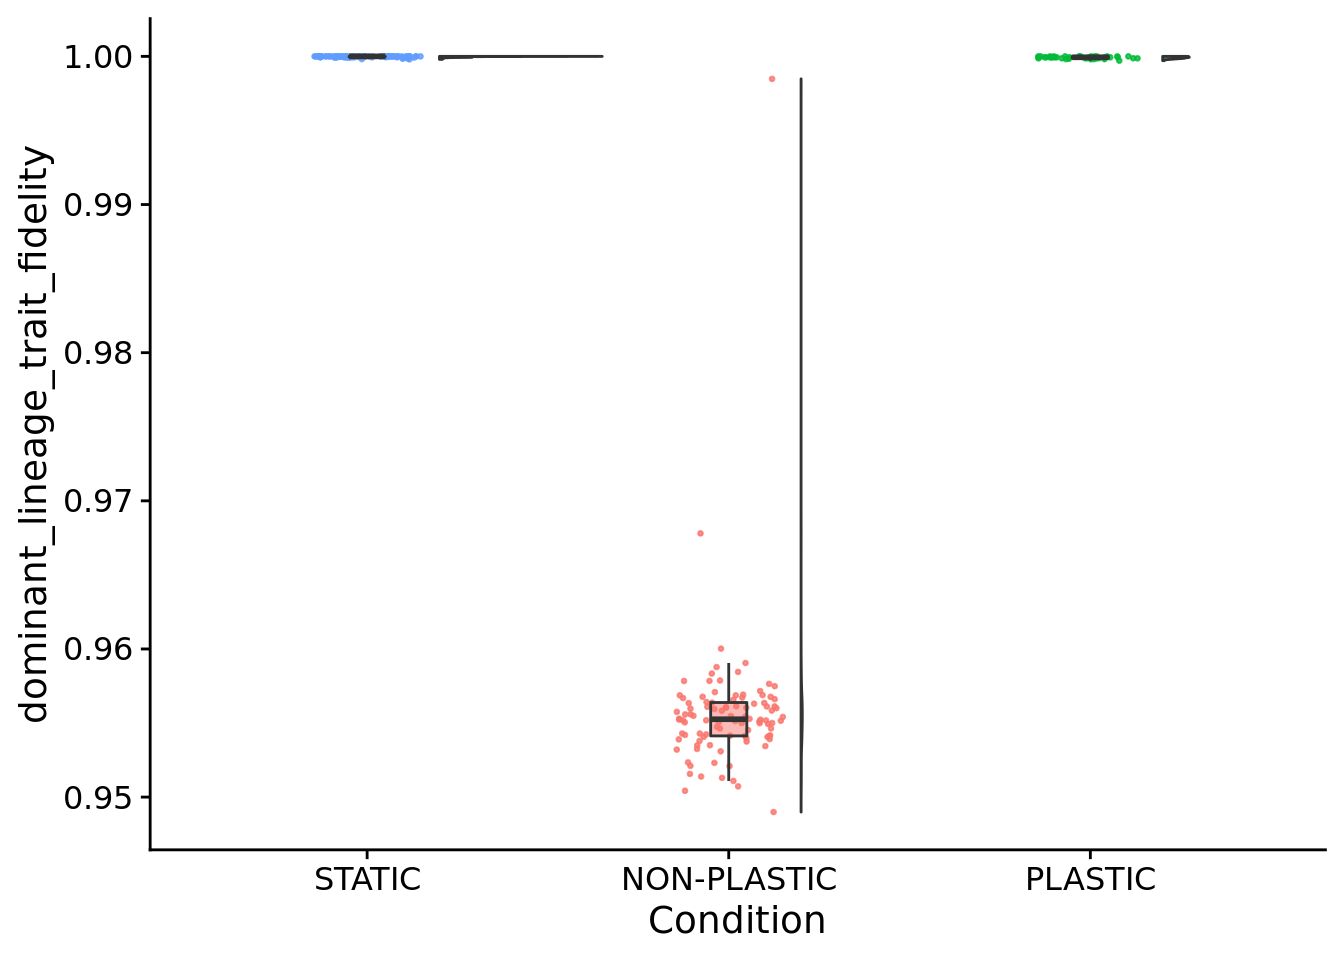
\includegraphics{supplemental-material_files/figure-latex/unnamed-chunk-25-1.pdf}

\bibliography{packages.bib,supplemental.bib}

\end{document}
